\documentclass[12pt]{jarticle}
\usepackage[dvipdfmx]{graphicx}
\usepackage{url}
\usepackage{listings,jlisting}
\usepackage{ascmac}
\usepackage{amsmath,amssymb}

%ここからソースコードの表示に関する設定
\lstset{
  basicstyle={\ttfamily},
  identifierstyle={\small},
  commentstyle={\smallitshape},
  keywordstyle={\small\bfseries},
  ndkeywordstyle={\small},
  stringstyle={\small\ttfamily},
  frame={tb},
  breaklines=true,
  columns=[l]{fullflexible},
  numbers=left,
  xrightmargin=0zw,
  xleftmargin=3zw,
  numberstyle={\scriptsize},
  stepnumber=1,
  numbersep=1zw,
  lineskip=-0.5ex
}
%ここまでソースコードの表示に関する設定

\title{知能プログラミング演習II 課題6}
\author{グループ8\\
  29114003 青山周平\\
  29114060 後藤拓也\\
  29114116 増田大輝\\
  29114142 湯浅範子\\
  29119016 小中祐希\\
}
\date{2019年1月6日}

\begin{document}
\maketitle

\paragraph{提出物} rep6
\paragraph{グループ} グループ8

\paragraph{担当}
\begin{tabular}{|c|l|}
  \hline
  氏名&担当課題\\
  \hline\hline
  青山周平&発展課題5-7の改良\\
  \hline
  後藤拓也&必須課題5-2の改良\\
  \hline
  増田大輝&発展課題5-5の改良\\
  \hline
  湯浅範子&必須課題5-4の改良\\
  \hline
  小中祐希&必須課題5-1の改良\\
  \hline
\end{tabular}

\section{課題の説明}
\begin{description}
\item[必須課題6-1] 課題5にやり残した発展課題があれば参考にして拡張しても良いし,全く新しい独自仕様を考案しても構わない.自由に拡張するか,あるいはもし残っていた問題点があれば完成度を高めよ.
\end{description}

\subsection{課題5の説明}
\begin{description}
\item[必須課題5-1] 目標集合を変えてみたときに,動作が正しくない場合があったかどうか,実行例を示して考察せよ.
また,もしあったならその箇所を修正し,どのように修正したか記せ.
\item[必須課題5-2] 教科書のプログラムでは,オペレータ間の競合解消戦略としてランダムなオペレータ選択を採用している.
これを,効果的な競合解消戦略に改良すべく考察し,実装せよ.
改良の結果,性能がどの程度向上したかを定量的に(つまり数字で)示すこと.
\item[必須課題5-3] 上記のプランニングのプログラムでは,ブロックの属性(たとえば色や形など)を考えていないので,色や形などの属性を扱えるようにせよ.ルールとして表現すること.
例えば色と形の両方を扱えるようにする場合,Aが青い三角形,Bが黄色の四角形,Cが緑の台形であったとする.
その時,色と形を使ってもゴールを指定できるようにする("green on blue" や"blue on box"のように)
\item[必須課題5-4] 上記5-2, 5-3で改良したプランニングシステムのGUIを実装せよ.
ブロック操作の過程をグラフィカルに可視化し,初期状態や目標状態をGUI上で変更できることが望ましい.
\item[発展課題5-5] ブロックワールド内における物理的制約条件をルールとして表現せよ.
例えば,三角錐(pyramid)の上には他のブロックを乗せられない等,その世界における物理的な制約を実現せよ.
\item[発展課題5-6] ユーザが自然言語(日本語や英語など)の命令文によってブロックを操作したり,初期状態/目標状態を変更したりできるようにせよ.
なお,命令文の動詞や語尾を1つの表現に決め打ちするのではなく,多様な表現を許容できることが望ましい.
\item[発展課題5-7] 3次元空間 (実世界) の物理的な挙動を考慮したブロックワールドにおけるプランニングを実現せよ.
なお,物理エンジン等を利用する場合,Java以外の言語のフレームワークを使って実現しても構わない.
\item[発展課題5-8] 教科書3.3節のプランニング手法を応用できそうなブロック操作以外のタスクをグループで話し合い,新たなプランニング課題を自由に設定せよ.
さらに,もし可能であれば,その自己設定課題を解くプランニングシステムを実装せよ.
\end{description}

\section{必須課題6-1(必須課題5-1の改良)}
\begin{screen}
目標集合を変えてみたときに,動作が正しくない場合があったかどうか,実行例を示して考察せよ.
また,もしあったならその箇所を修正し,どのように修正したか記せ.
\end{screen}
\begin{screen}
課題5にやり残した発展課題があれば参考にして拡張しても良いし,全く新しい独自仕様を考案しても構わない.自由に拡張するか,あるいはもし残っていた問題点があれば完成度を高めよ.
\end{screen}
前レポートにおいて課題5-1では,目標状態の順番が不適切である場合に適切な順番に直すというメソッドを実装した.具体的にいうと、例えばAonB,BonCのような順番でリストに入っている場合AonBが先に対象となってしまい,積木の上の部分が先に完成してしまい残りの推論がうまくいかなくなるということが起こるため,リスト内の順番をより下になるブロックを含む目標状態が先に来るように並べ替えるというものであった.\\
前レポートではこのメソッドを実装した上でプログラムを実行したのだが,他の箇所との連携等の問題から実際には機能していないにもかかわらず実行結果だけがうまく出てしまっていたことがわかった.また,メソッド単体での検証をしていなかったのでメソッド自体の有用性も確認できていない事になる.\\
そこで,本レポートではメソッドの検証及び不具合の解消を行うこととする.

\subsection{検証}
まず,前回作成したメソッドを単体で実行できるように別途プログラムを作成した.\\
目標状態を(A on B)(B on C)(C on D)で実行したところ,以下のような実行結果が得られた.

\begin{lstlisting}[caption=修正前プログラム, label=mid]
head[0]A
tail[0]B
head[1]B
tail[1]C
head[2]C
tail[2]D
initGoalList = [A on B, B on C, C on D]
goalList = [A on B, B on C, C on D]
\end{lstlisting}
リストhead,tailはそれぞれ目標状態の先頭と末尾の文字を格納したリストであり,initGoalListはメソッドへの引数(変更前),goalListはメソッドの返り値(変更後)である.\\
このことから,メソッドがうまく機能していないことがわかった.

\subsection{手法}
ハンドトレースをした限りではうまく機能する見込みがあったので,ひとまずアルゴリズムはそのままにしていわゆるバグ探しの作業を行った.\\
原因となっている箇所を見つけ出すために番号を出力するprint文をプログラムの各重要箇所に配置して再度実行をかけたところ,先頭の文字と末尾の文字が一致するかという分岐のところで先に進んでおらず,全てif文をスルーしてしまった結果一切入れ替えが行われていなかった.\\
結論としては,分岐の判定で等価演算子を使ってしまっていたことが原因出会った.よって,if文の条件式をtail[i].equals(head[j])と変更した.

\subsection{実装}
以下に,検証用のパーツ含め修正したメソッド全体を示す.\\

\begin{lstlisting}[caption=修正後プログラム, label=mid]
public static ArrayList<String> sortGoalList(ArrayList<String> goalList) {
		ArrayList<String> sortedGoalList = new ArrayList<String>();

		//sortedGoalListに目標状態を格納
		for(String s : goalList) {
			sortedGoalList.add(s);
		}

		for(int k = 0; k < sortedGoalList.size(); k++){
			String[] head = new String[sortedGoalList.size()];
			String[] tail = new String[sortedGoalList.size()];

			//各目標状態の先頭と末尾の文字を配列に格納
			for(int i = 0; i < sortedGoalList.size(); i++){
				head[i] = sortedGoalList.get(i).substring(0,1);
				tail[i] = sortedGoalList.get(i).substring(sortedGoalList.get(i).length()-1);
			}
			

			//headとtailを出力
			for(int i = 0; i < head.length; i++) {
				System.out.println("head["+i+"]"+head[i]);
				System.out.println("tail["+i+"]"+tail[i]);
				System.out.println();
			}


			int flag = 0;
			//System.out.println(0);
			for(int i = 0; i < sortedGoalList.size(); i++){
				//System.out.println(1);
				for(int j = i; j < sortedGoalList.size()-i; j++){
					//System.out.println(2);
					if(tail[i].equals(head[j])){
						//System.out.println(3);
						sortedGoalList.add(j+1, sortedGoalList.get(i));
						sortedGoalList.remove(i);
						//System.out.println("i="+i+" j="+j+" list= "+sortedGoalList);
						flag += 1;
						break;
					}
				}
				if(flag == 1){
					break;
				}			
			}
			if(flag == 0){
				break;
			}

		}

		return sortedGoalList;
	}
\end{lstlisting}

\subsection{実行例}
修正の結果,以下のような結果が得られた.
\begin{lstlisting}[caption=実行結果, label=mid]
head[0]A
tail[0]B

head[1]B
tail[1]C

head[2]C
tail[2]D

head[0]B
tail[0]C

head[1]A
tail[1]B

head[2]C
tail[2]D

head[0]A
tail[0]B

head[1]C
tail[1]D

head[2]B
tail[2]C

initGoalList = [A on B, B on C, C on D]
goalList = [C on D, B on C, A on B]
\end{lstlisting}


\subsection{考察}
ここでは,今回のようにメソッドが機能していないにもかかわらず,機能しているように見えてしまったことについて考察する.前回にレポートで作成したsortGoalListメソッドは,目標状態の順番により推論機能がうまく機能しないという現象を解消するために実装したものである.したがって,目標状態はどんな状態でも機能することを目標としており,目標状態は元々用意されていたinitGoalListから取得するようにしてあった.\\
しかしながら,本課題において私の班はGUIを実装する手段としてプレゼンターを用意しており,プレゼンターは直接Planner.javaのメソッドにアクセスする形になっている.その結果,他の課題を実装する過程で目標状態に関して直接initGoalListから目標状態を取得するようになっており,作成したsortGoalListメソッドが機能していない状態になってしまっていたと考えられる.\\



\section{必須課題6-1(必須課題5-2の改良)}
\begin{screen}
課題5にやり残した発展課題があれば参考にして拡張しても良いし,全く新しい独自仕様を考案しても構わない.自由に拡張するか,あるいはもし残っていた問題点があれば完成度を高めよ.
\end{screen}
\subsection{前回の内容}
\begin{screen}
教科書のプログラムでは,オペレータ間の競合解消戦略としてランダムなオペレータ選択を採用している.
これを,効果的な競合解消戦略に改良すべく考察し,実装せよ.
\end{screen}
前回の課題5-2では, 「Place A on A(存在しない制約)」や「Place B on A(属性を考量した場合の禁止制約)」を改良させるために, 属性クラスであるAttributionsクラスで定義した禁止制約のXonY関係をHashMapに格納し, その条件と現状態のX'onY'関係を照らし合わせるという方法を用いた. オペレータ選択にはランダム選択を用いることで, どんなに適当な状態になっても禁止制約が発動されることを保証するようにした. \\

実行結果は以下のように失敗していた.
\begin{lstlisting}[caption=失敗実行例その1, label=src:No1]
*** GOALS ***[holding B]
**holding B
そのオペレータは実行できません
おすすめのオペレータを使います
**clear ?y3
[clear A, clear B, clear C, ontable A, ontable B, ontable C, ontable pyramid, handEmpty]
*** GOALS ***[holding B]
**holding B
そのオペレータは実行できません
おすすめのオペレータを使います
**clear ?y3
[clear A, clear B, clear C, ontable A, ontable B, ontable C, ontable pyramid, handEmpty]
*** GOALS ***[holding B]
**holding B
そのオペレータは実行できません
おすすめのオペレータを使います
**clear ?y3
...(以下無限に続く)
\end{lstlisting}

問題点としては, 離れた制約がうまく機能していなかったことである. 「B on ?y1」という目標に対して, オペレータ「Place ?x2 on ?y2」によって, 「?x2 = B」と「?y2 = ?y1」となるのはよいが, その後, 「Clear A」と「Clear ?y2」のマッチングを行う際に, 「?y2 = ?y1 = A」となるが, この処理において, 禁止制約(X on Y関係)との関係がうまく取れていなかったのである. 以下の図1を参照してほしい.

% ここに図1を作って説明
\begin{figure}[htbp]
 \begin{center}
  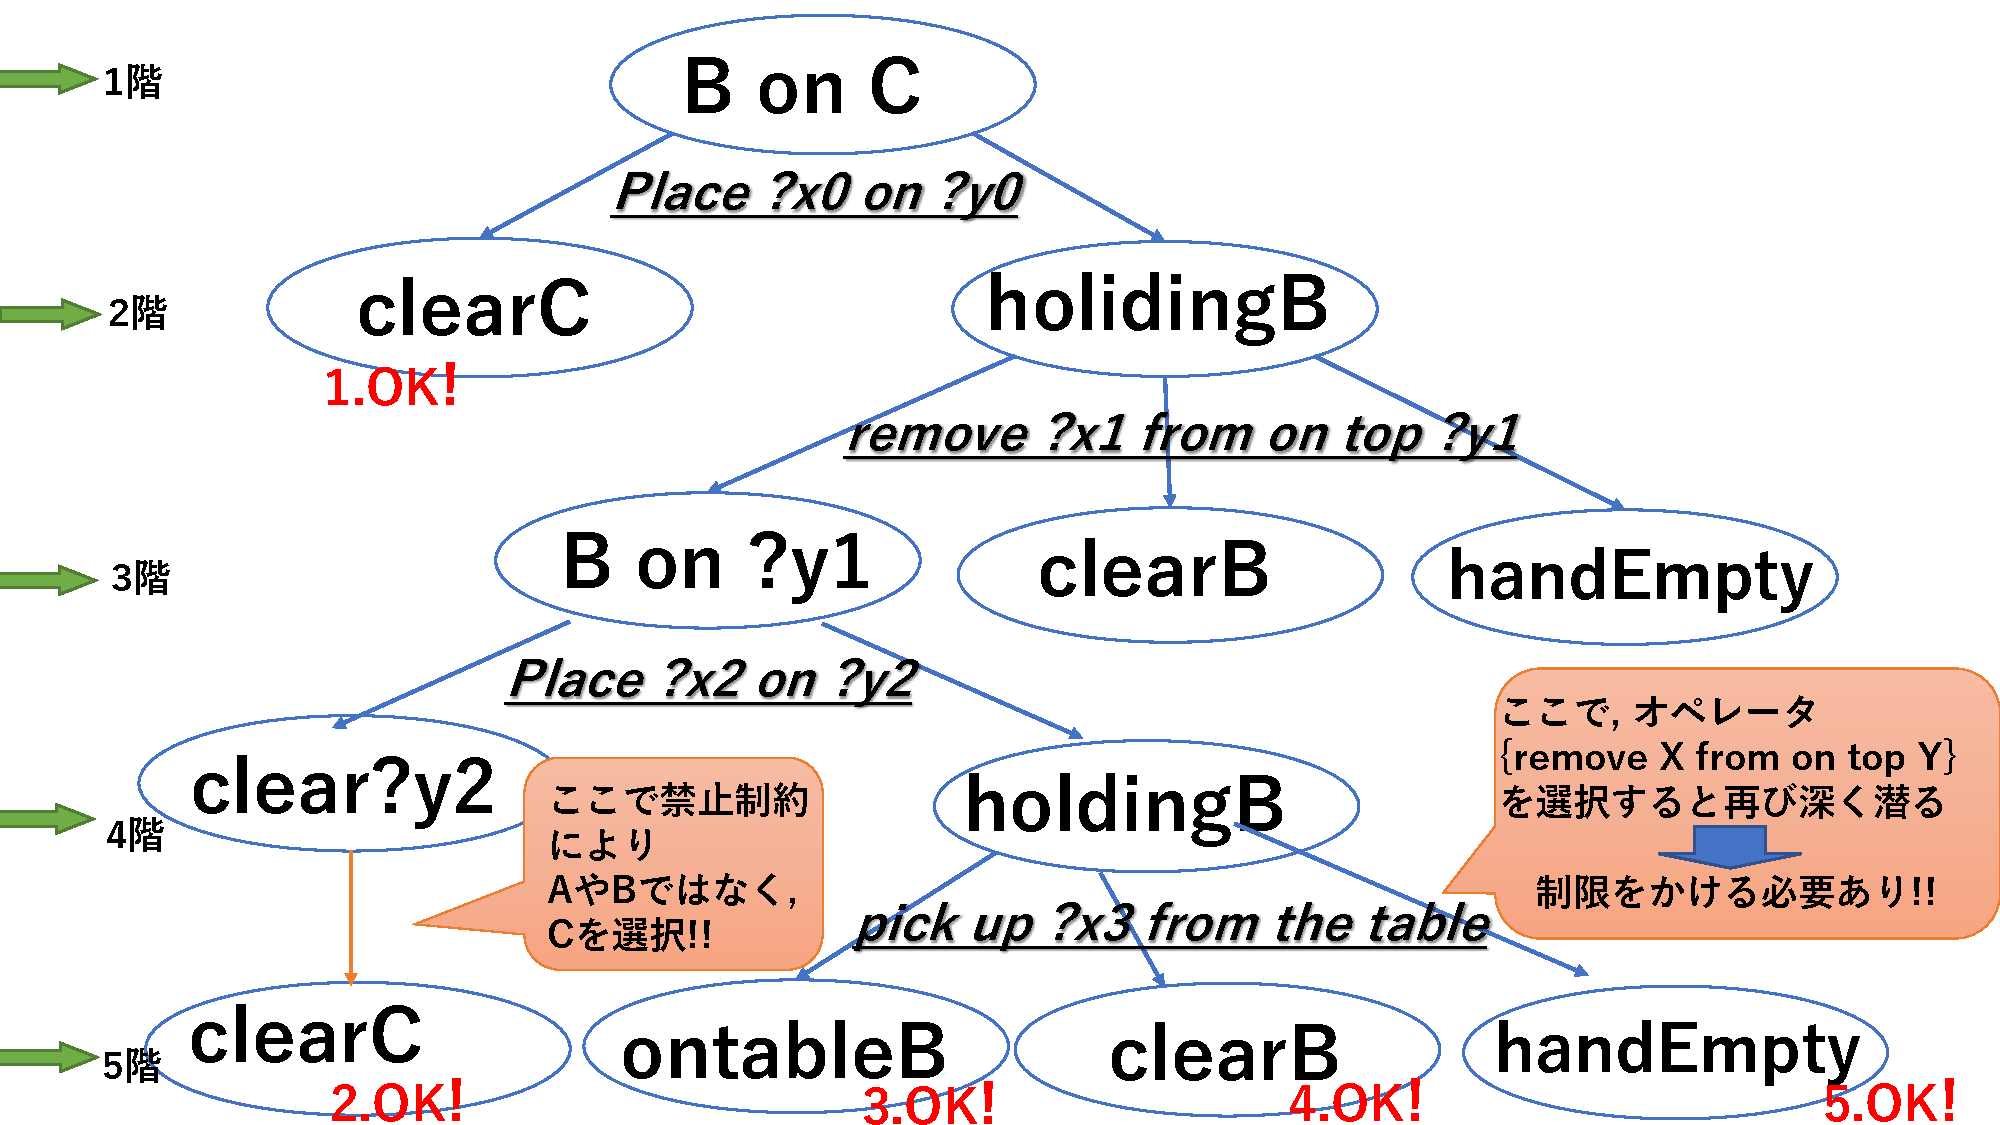
\includegraphics[width = 12cm, pagebox = cropbox, clip]{images/treeContsraction.pdf}
 \end{center}
 \caption[]{plannnigの再帰呼び出しの木構造表現}\label{fig:fig1.1}
\end{figure}

初期設定から与えられる禁止制約:prohibitと, 現在の状態を表す:productKeyOnValueを照らし合わせて, 積み方に制約をかけている. productKeyOnValueには, 「X on Y関係」の目標が生じたときに, 現在問題にしている「X on Y関係」の何がXで何がYかを保存する. これは, 上記で述べたような離れた制約(B on ?y1の後に,Clear ?y2など)にも対応できるようにするためである.

これを実装するにあたり, replaceBufferのタイミングも変更した. 以前のプログラムの内容では, 「?x1 = A」と決まった後で, 「?x2 = A」と制約を加える形をとっていた. それでは, ?x2 = ?x1の対応が取れない.(実装で内容を詳しく説明)\\ % なげやりやね・・・

% 木を図2を用いて表現
また, 木構造を用いてこれらの再帰構造の内容を表現すると図2のようになる.
図2は, 目標「B on C, A on B」における「B on A」を単体目標としたときの再帰構造の様子である. 1階の「B on C」に対して, オペレータ「Place ?x on ?y」のadd部がマッチングし, そのif部が次の目標となり, 1つ深くなり, 2階目へ移行する. その後同様の処理を深さ優先探索として行われる.

ここでポイントになるのは, 「X on Y関係」において, 1階と2階の間で決定される「?x0 on ?y0関係」に対して, 3階で定義される「B on ?y1」関係においては, 4階で決定されるのではなく, 5階で決定される. このように3階で定義されたものが次の階ではなく, 5階で定義される状態を"離れた制約"と呼んでいる. 前回のプログラムではこの点に関してうまくいっていなかった. 今回はこの点を修正した. 実装方法は前回の内容を利用し, 以下のように変更を加えた.

%実装方法の説明
\subsection{実装}
Attribuiteクラスで定義された禁止制約(A on Aなど)をHashMapに格納し, それをPlannerクラスで呼び, Unifierクラスとその情報を共有する. そして現在の「X on Y関係」を保存するHashMap:productKeyOnValueを用いて禁止制約との照らし合わせをする. 以下には前回の実装では失敗していたUnifierクラスでの"禁止制約との照らし合わせによるマッチング"を示す.
\begin{lstlisting}[caption=UnifierクラスのvarMatchingメソッド, label=src:No1]
boolean varMatching(String vartoken, String token) {
 System.out.println("vars="+vars);
 System.out.println("vartoken="+vartoken);
 System.out.println("token="+token);
 if(vars.containsKey(vartoken)) {
   if(token.equals(vars.get(vartoken))) {
	return true;
   }else{
	return false;
   }
 }else{
   /* ココじゃなくて...
   replaceBuffer(vartoken, token);
   if (vars.containsValue(vartoken)) {
      replaceBindings(vartoken, token);
   }
   */
   if(productKeyOnValue != null) {
      //product_KeyValueの数
      for(String str1 : productKeyOnValue.keySet()){	
	   System.out.println("vars="+vars);
	   if(var(productKeyOnValue.get(str1))) {
		for(int num=0; num<prohibit.get(str1).size(); num++) {
		    if(vars.containsKey(productKeyOnValue.get(str1))) {
		     System.out.println(productKeyOnValue.get(str1));
		     if(vars.get(productKeyOnValue.get(str1)).equals(vartoken) & prohibit.get(str1).get(num).equals(token)){
			   System.out.println("禁止制約発動しました.");
			   return false;
			}
		     }
	       }
	     }
      }
   }
  //ココで行います!
  replaceBuffer(vartoken, token);
  if (vars.containsValue(vartoken)) {
	replaceBindings(vartoken, token);
  }
	vars.put(vartoken, token);
  }
  return true;
}
\end{lstlisting}

上記のプログラムでは自分でも何をやっているのかわからなくなるので以下の図2, 図3を参考にしながらプログラムを見ていただきたい.

% 図2 プログラムの内容
\begin{figure}[htpb]
  \centering
    \begin{tabular}{c} 
      \begin{minipage}{0.50\hsize}
        \centering
          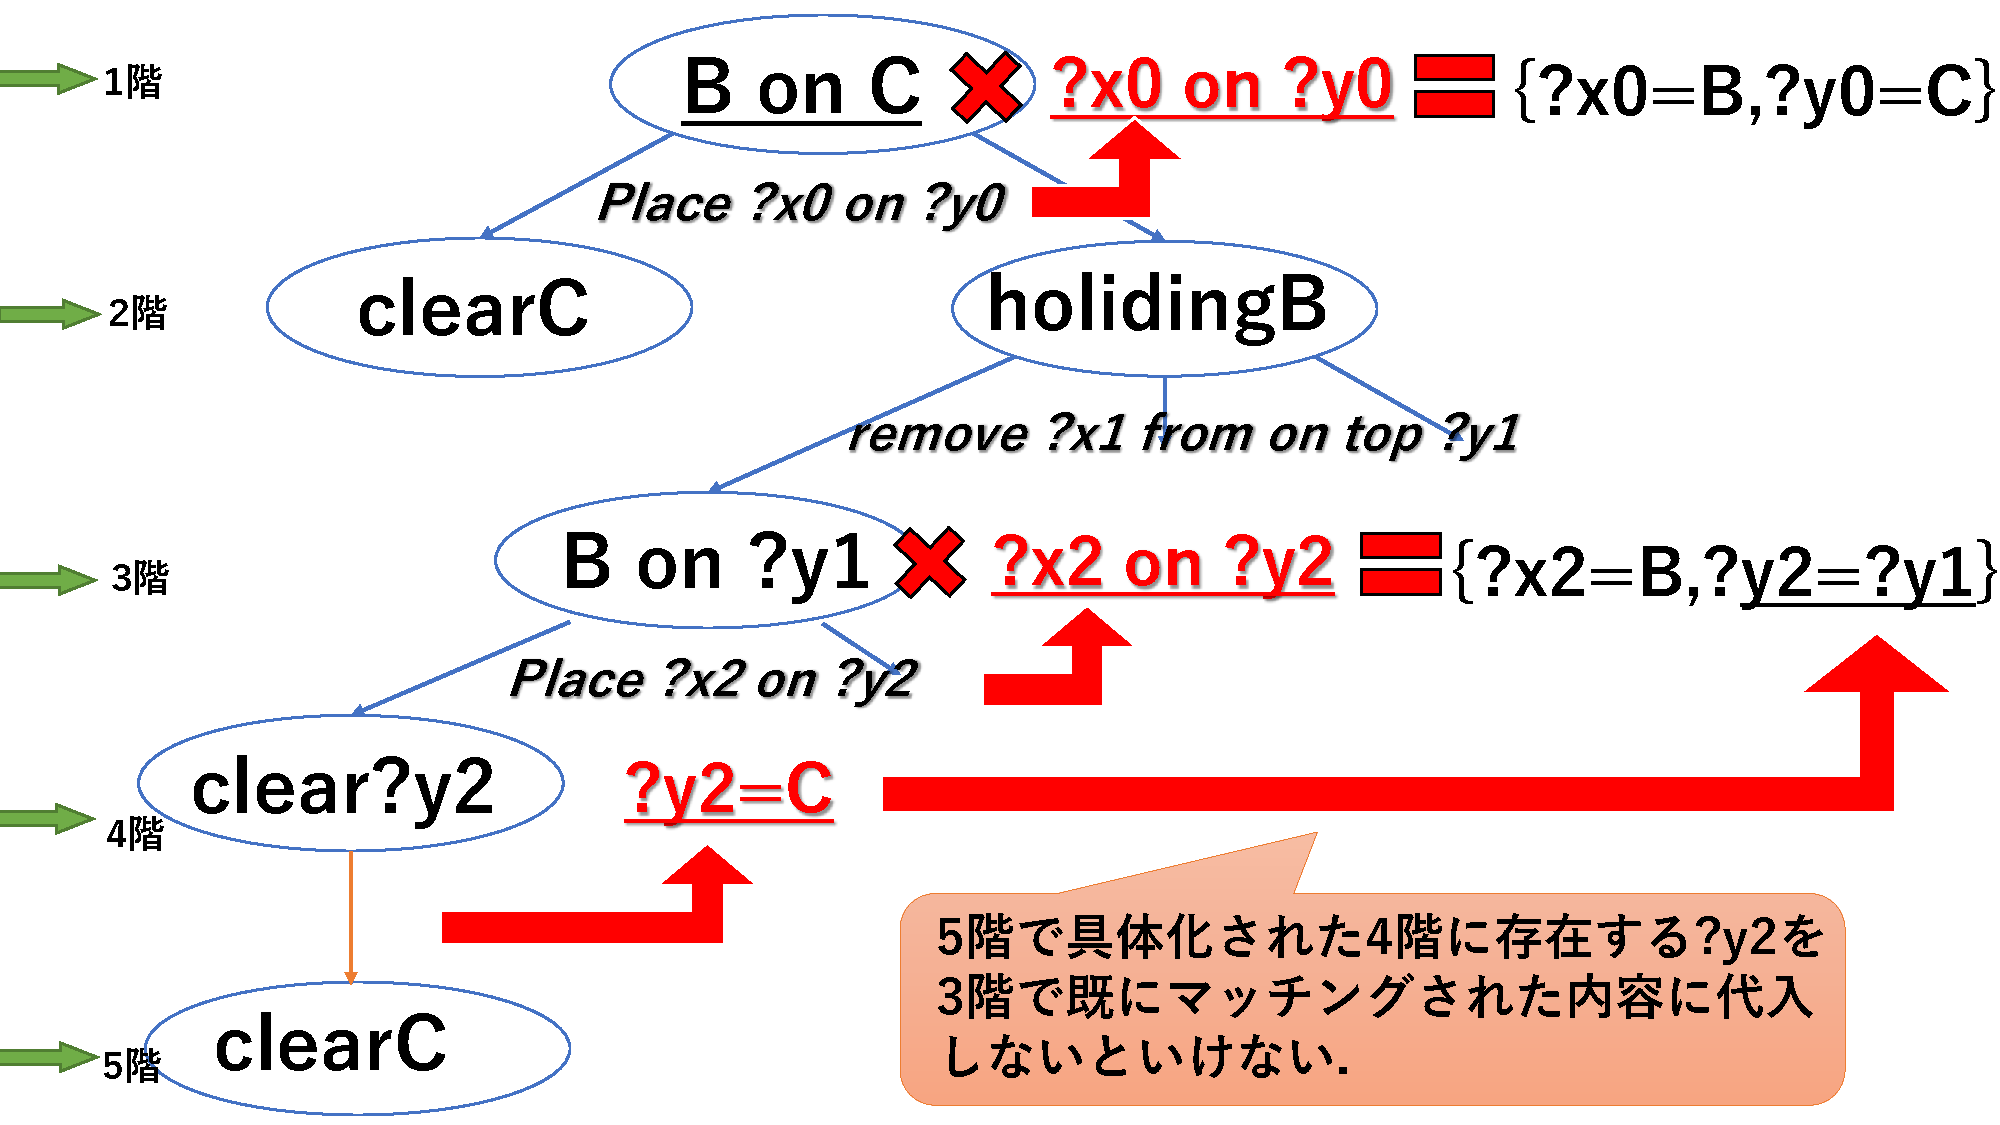
\includegraphics[width = 6.5cm, pagebox = cropbox, clip]
                          {images/treeSupplement.pdf}
                          \caption{階層的な視点}
                          \label{fig:1.3}
      \end{minipage}
 
      \begin{minipage}{0.50\hsize}
        \centering
          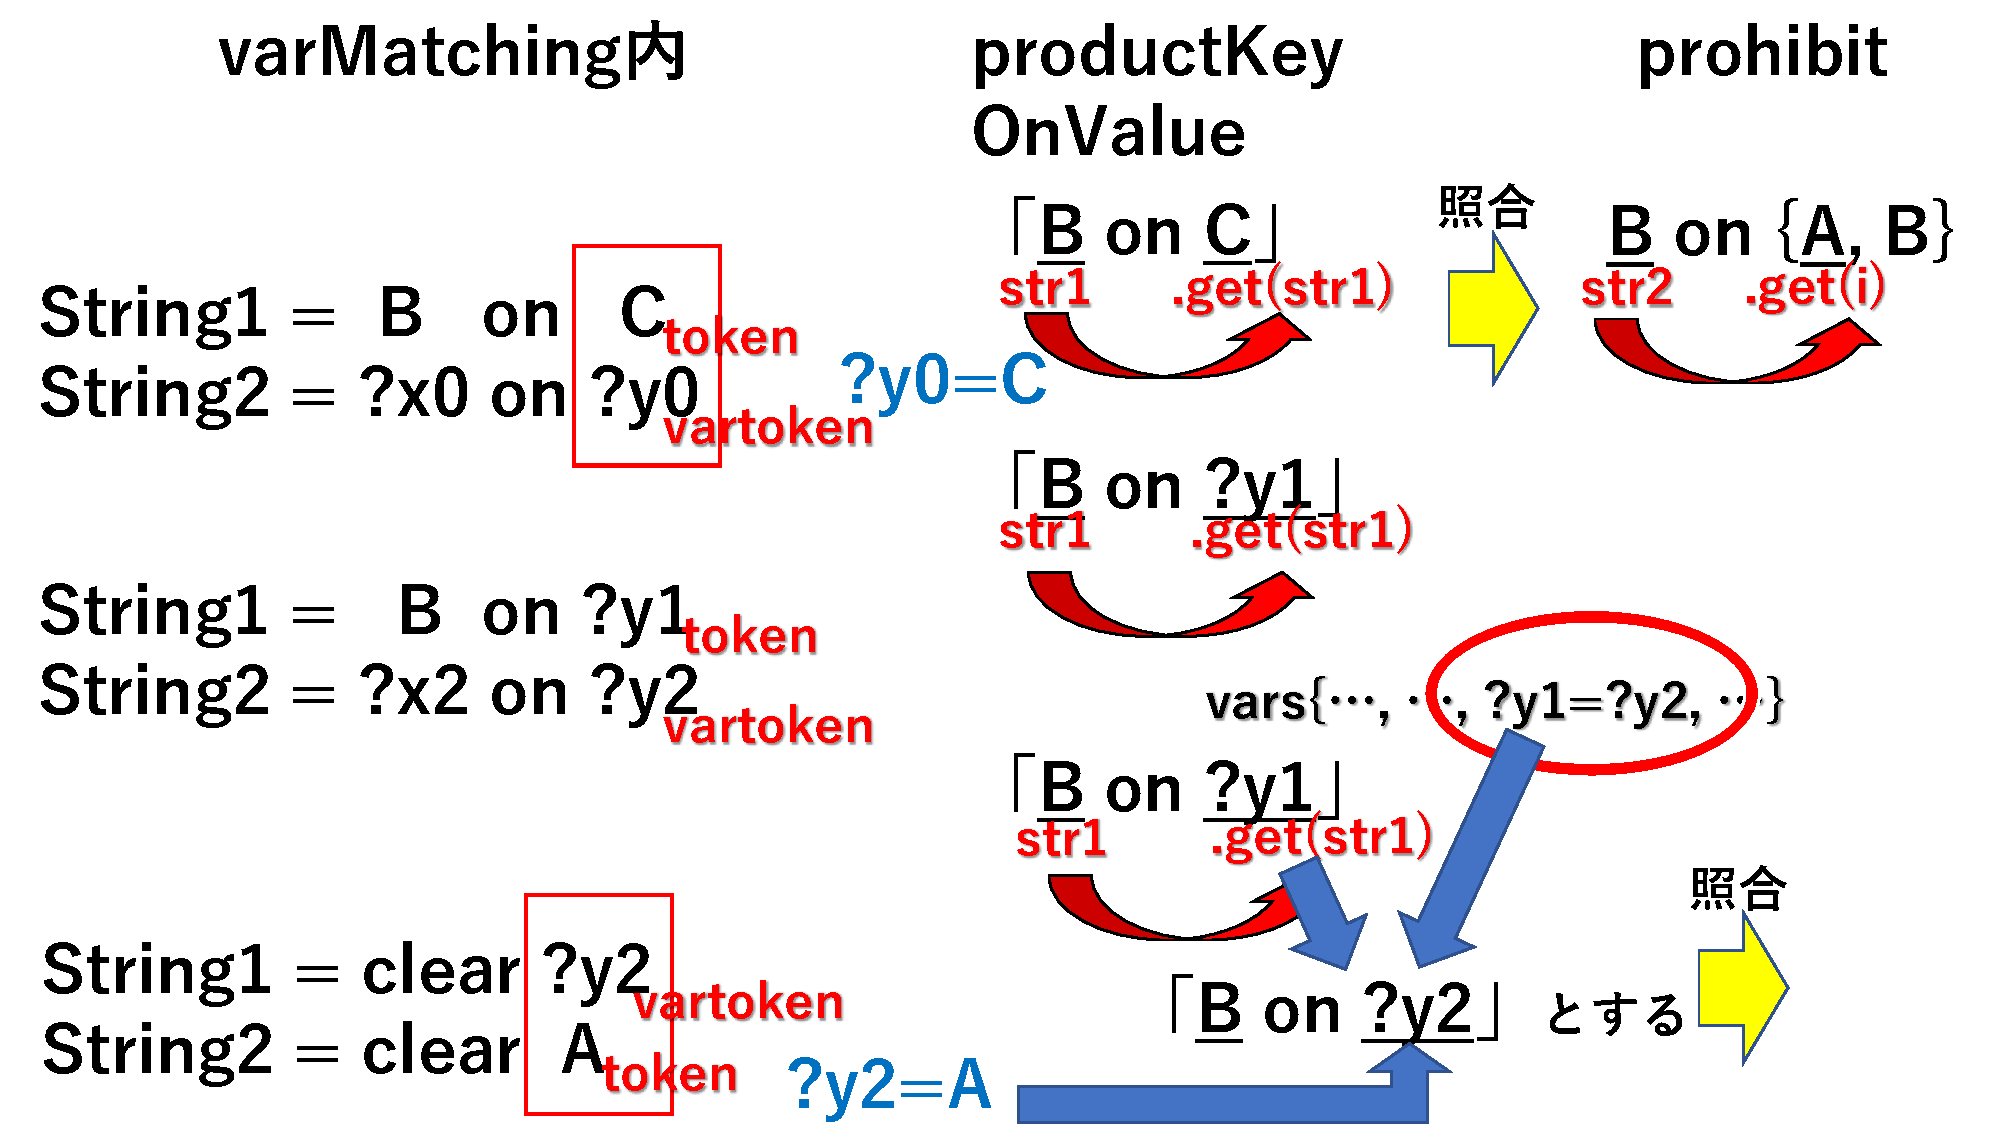
\includegraphics[width = 6.5cm, pagebox = cropbox, clip]
                          {images/varMatching.pdf}
                          \caption{varMatching内の処理内容}
                          \label{fig:1.3}
      \end{minipage} \\ 
    \end{tabular}
\end{figure}     

図2, 3ともに, 「X on Y関係」だけに焦点を絞っている. 図2からは, 「?x0 on ?y0」の場合に2階から1階へのマッチングに対し, 「?x2 on ?y2」の場合は, 5階の「clearC」のCを使って, 3階のマッチングに利用されていることを示している. 図3は, UnifierクラスのVarMatchingメソッド内でのマッチングする2つの文, 現状態XonY関係を示すHashMap:productKeyOnValue, 禁止制約のHashMap:prohibitが示されている. \\

図2の各階のノードが決定された時点で, 図3のproductKeyOnValueにはそのノードの値が代入され, その後, 選択されたオペレータのadd部(X on Yに絞って言及中)とMatchingをする. productKeyOnValueもprohibitも, HashMapなので, 「X on Y」が「Key on Value」の関係で呼び出すことができる. 1,2階間でのマッチング処理は, varMatchingメソッドでマッチングした?x0, ?y0をそのままprohibitの禁止制約と照らし合わせればよいが, 3~5階間でのマッチング処理は, 図2のノードはあくまで, 「B on ?y1」なので, ?y2との関係は「B on ?y1」と「?x2 on ?y2」のマッチングが終わった後に確定される. その関係はハッシュマップ:varsに格納されるので, それを用いて, ノードの「B on ?y1」を「B on ?y2」とする. そして, 4~5階で?y2=Cとマッチングすると, その情報を現状態のノード:productKeyOnValueに代入することで, 「B on A」という関係を生成させる. それと禁止制約を照合することで, 多階層のX on Y関係でも対応できるようにした. プログラムのfor文では, productKeyOnValueのKey値(str1)とVlaue値(.get(str1))を見て, そのKey(str1)に対応する禁止制約のprohibitのVlaue値(.get(str2))をもってきたのち, ifの条件文で, HashMap:varsの{?y1=?y2}関係と禁止制約:prohibitのvalue値を1つずつ照らし合わせる処理をしている.\\

そして以上のvarsの関係[?y1=?y2]の関係を見た後で, ?y2=Cとし, ?y1=Cとするところから, replaceBufferメソッドの呼び出しは, 上記の内容を行った後で実行するようにした. 先にreplaceBufferメソッド呼び出してしまうと, Key:?y1のValue値は?y2となってしまい, 具体化されないまま終わってしまうからである.


\subsection{実行例}
今回の実行においては, 上記の説明を実際に表示させるために, オペレータの選択を自分で選択し, 逐一状況を確認していく.
\begin{lstlisting}[caption=3~5階層のマッチング, label=src:No1]
Place ?x2 on ?y2
addList = [?x2 on ?y2, clear ?x2, handEmpty]
string1=B on ?y1
string2=?x2 on ?y2
productKeyOnValue保存 = {B=?y1}
vars={?y0=C, ?x0=B, ?x1=B}
vartoken=?x2
token=B
productKeyOnValue.get()=?y1
vars={?y0=C, ?x0=B, ?x1=B}
vars={?y0=C, ?x0=B, ?x1=B, ?x2=B}
vartoken=?y1
token=?y2
productKeyOnValue.get()=?y1
vars={?y0=C, ?x0=B, ?x1=B, ?x2=B}
その2
Key = B Value = ?y1
unify成功
オペレータの具体化:Place B on ?y2
*** GOALS ***[clear ?y2, holding B]
**clear ?y2
string1=clear ?y2
string2=clear A
vars={?y0=C, ?x0=B, ?y1=?y2, ?x1=B, ?x2=B}
vartoken=?y2
token=A
productKeyOnValue.get()=?y1
vars={?y0=C, ?x0=B, ?y1=?y2, ?x1=B, ?x2=B}
禁止制約発動しました.
string1=clear ?y2
string2=clear B
vars={?y0=C, ?x0=B, ?y1=?y2, ?x1=B, ?x2=B}
vartoken=?y2
token=B
productKeyOnValue.get()=?y1
vars={?y0=C, ?x0=B, ?y1=?y2, ?x1=B, ?x2=B}
禁止制約発動しました.
string1=clear ?y2
string2=clear C
vars={?y0=C, ?x0=B, ?y1=?y2, ?x1=B, ?x2=B}
vartoken=?y2
token=C
productKeyOnValue.get()=?y1
vars={?y0=C, ?x0=B, ?y1=?y2, ?x1=B, ?x2=B}
theBinding{?y0=C, ?x0=B, ?y1=C, ?x1=B, ?y2=C, ?x2=B}
\end{lstlisting}

「?x2 on ?y2」関係から「clear C」に至るまでの処理を図2,3を参考にしながら見ていただけると, よくわかると思う. 「B on A」という禁止制約が発動され, A, Bではマッチングが行われず, Cのみで成功している. 実際に, 最後のBinding情報では, {?y1=C,...,?y2=C}と正しく行われていることが分かる.

\subsection{考察}
図1の木構造からも分かるように, 問題に上がっていた繰り返しの処理(Place A on B, remove A from on top Bの繰り返し)をなくすには, 「pick up B from the table」を選択するしかないということが分かる.

ただ, 以下の実行結果を見てもらいたい. 最終結果のみを記す.
% 「A on C」という実行結果
\begin{lstlisting}[caption=A on Cが生じてしまう, label=src:No1]
***** This is a plan! *****
pick up B from the table
Place B on C
remove B from on top C
Place B on C
pick up A from the table
Place A on C
remove A from on top C
Place A on B
\end{lstlisting}


確かに, 「A on C」という禁止制約は存在しないが, 既に「B on C」が存在している状況で, 「A on C」とすることは...物理的に不可能である. そのため, 実行中にも, 禁止制約を随時追加していかなければならないことが分かる. ただ, 「B on C」が確定したのちに「A on C」はダメという禁止制約, 「remove B from on top C」を実行された後には, 「A on C」はダメではないので禁止制約から取り除くといった処理を行うのは, また...大変であり, planningの実装に向けては, かなりゲームフィールの制限を強くするしかないことが分かった. "知識システム"の授業で, 新谷先生が「条件を限定した仮想空間を用いないとプログラムに書ききらないよ」と言っていた内容が良く分かった.


\section{必須課題5-2のさらなる改良}
\subsection{序論}
上記では, 禁止制約を「X on Y関係」のHashMapを用いることで解決するアプローチを試みた. その際に, 図1で紹介したが, 「AをとってBの上に置く」, 「AをBから取り除く」, 「AをとってBの上に置く」, 「AをBから取り除く」といった無駄な処理をなくす方法として, オペレータの選択に制限をかける必要があると述べた. 今回はそのプログラムを実装してみる.

\subsection{手法}
図1でもわかるように, 2階で「holdingB」という目標が設定されていて, その後, 4階でも同じ「holdingB」という目標が出てくる. 4階で2階と同じオペレータ(ここでは, remove X from on top Y)を選択したらどんどんと木は深くなる. そのため, planningAGoalメソッドで設定された1つの目標(木構造におけるノード)と, そのノードに対して選択されたオペレータを保存しておき, 繰り返しを防ぐという方法をとる.

\subsection{実装}
Plannerクラスに, 1つの目標(木構造におけるノード)とその時に選択されたオペレータの対応関係を保存するHashMap:goalOpを作成. Keyには目標, Valueにはオペレータのインデント[0~3]を保存する. (オペレータの選択とインデントの関係に関しては, 課題5のレポートを参照してもらいたい.)

\begin{lstlisting}[caption=目標とオペレータの対応関係の保存, label=src:No1]
//Plannerクラス
  HashMap<String, Integer> goalOp;	//Key:単目標/Value:オペレータの番号
//コンストラクタ
  goalOp = new HashMap<String, Integer>();

//planningAGoalメソッド内
  //1.stateリストとの照らし合わせ処理(省略) 
  //2.ノードをKeyとして保存(Value)は未定値
  if(!goalOp.containsKey(theGoal)) {
    goalOp.put(theGoal, -1);
  }
  //3.operatorの選択(ランダム)
  int randInt = Math.abs(rand.nextInt())\%operators.size();
  Operator op = (Operator)operators.get(randInt);
  cPoint = randInt;
  //4-1.選択したオペレータの実行(一部省略)
  Operator anOperator = rename((Operator) operators.get(cPoint));
  for (int j = 0; j < addList.size(); j++) {
    Unifier unification = new Unifier();
    if(unification.unify(theGoal, (String) addList.get(j), theBinding, attributions.keyValueProhibit, p_productKeyOnValue)) {
      //5.一度は選択されていたら,break
      if(goalOp.get(theGoal) == cPoint) {
        System.out.println("breakします");
	  break;
      }
      //6.breakしなかったら, 保存する
      goalOp.put(theGoal, cPoint);
      System.out.println("goalOp"+goalOp);
	...
  //4-2.選択されたオペレータが実行されない場合,
  for (int i = 0; i < operators.size(); i++) {
    if(i != cPoint) {
    anOperator = rename((Operator) operators.get(i));
    addList = (ArrayList<String>) anOperator.getAddList();
    for (int j = 0; j < addList.size(); j++) {
      Unifier unification = new Unifier();
	if(unification.unify(theGoal, (String) addList.get(j), theBinding, attributions.keyValueProhibit, p_productKeyOnValue)) {
     //5.既にその目標に対してオペレータが選択されていたら,
	  if(goalOp.get(theGoal) == i) {
             System.out.println("breakします");
		break;
          }
     //6.保存する
	goalOp.put(theGoal, i);
	System.out.println("goalOp"+goalOp);
	...
\end{lstlisting}

選択したオペレータが実際に実行されるか, それとも別のオペレータが実行されるかに関しては, 課題5のレポートを参考にしてもらいたい.

planningAGoalメソッドが実行されたら, まず, HashMap:goalOpにその目標がKeyとして設定されていない場合は, Valueを-1としておく. それ以前にすでにその目標がKeyとして保存されていたら, -1の初期化は行わない. その後, 実際に, オペレータのadd部とunifyをしていき, 成功したら, そのオペレータのインデントをgoalOpのValueに加える(上書き保存する). すでにその目標に対して, 以前実行されたオペレータがあり, 保存されていたら(つまり-1ではなかったら), 別のオペレータを探すためにfor文をbreakし, 下の"選択されたオペレータ以外のオペレータの実行" へ移動する. そこで, 一度も選択されていないオペレータだったら, そのオペレータを実行する.

\subsection{実行結果}
\begin{lstlisting}[caption=goalOpによって制約される , label=src:No1]
[B on C, A on B]
*** GOALS ***[B on C, A on B]
**B on C
Place ?x0 on ?y0
goalOp{B on C=0}
*** GOALS ***[clear C, holding B]
**clear C
theBinding{?y0=C, ?x0=B}
*** GOALS ***[holding B]
**holding B
remove ?x1 from on top ?y1
goalOp{holding B=1, B on C=0}
オペレータの具体化:remove B from on top ?y1
*** GOALS ***[B on ?y1, clear B, handEmpty]
**B on ?y1
Place ?x2 on ?y2
goalOp{holding B=1, B on C=0, B on ?y1=0}
オペレータの具体化:Place B on ?y2
*** GOALS ***[clear ?y2, holding B]
**clear ?y2
theBinding{?y0=C, ?x0=B, ?y1=C, ?x1=B, ?y2=C, ?x2=B}
*** GOALS ***[holding B]
**holding B
Place ?x3 on ?y3
そのオペレータは実行できません
remove ?x4 from on top ?y4
breakします
pick up ?x5 from the table
オペレータの具体化:pick up B from the table
*** GOALS ***[ontable B, clear B, handEmpty]
**ontable B
theBinding{?y0=C, ?x0=B, ?y1=C, ?x1=B, ?y2=C, ?x2=B, ?x4=B, ?x5=B}
*** GOALS ***[clear B, handEmpty]
**clear B
theBinding{?y0=C, ?x0=B, ?y1=C, ?x1=B, ?y2=C, ?x2=B, ?x4=B, ?x5=B}
*** GOALS ***[handEmpty]
**handEmpty
theBinding{?y0=C, ?x0=B, ?y1=C, ?x1=B, ?y2=C, ?x2=B, ?x4=B, ?x5=B}
Success !
Success !
Success !
...
\end{lstlisting}

「holdingB」が2回目の目標として設定された際に, 「Place ?x3 on ?y3」のオペレータを選択しているが, add文には「holdingX」が存在しないので, 次のオペレータを探す. すると, 「remove ?x4 from on top ?y4」が選択されるが, goalOpにすでに{holding B=1}と保存されているので, インデント1のremoveオペレータは実行されない. その後, 「pick up ?x5 from the table」が実行され, 成功していることが分かる.

\subsection{考察}
このプログラムにより, オペレータの選択をランダムにしても, 無駄な処理(AをBの上に置いて, AをBから取り除いて, またAをBの上において...など)はなくなった. 完璧なプログラムかといえば, 結局, 「Place A on C」という前に述べた"物理的に不可能な置き方"が残ってしまったので, 残念である. また, "机に置いてある3つの積み木(A, B, C)を順に上に積んでいく"という処理しかできなくなり, 汎用性がなくなってしまった. 本当は積み木が4つになって, 初期状態がどうであれ, 最終的な目標状態がどうであれ, 適切なオペレータ選択ができればよかったが, なかなか難しい...



\section{必須課題6-1(必須課題5-4の改良)}
\begin{screen}
上記5-2, 5-3で改良したプランニングシステムのGUIを実装せよ.
ブロック操作の過程をグラフィカルに可視化し,初期状態や目標状態をGUI上で変更できることが望ましい.
\end{screen}
\begin{screen}
課題5にやり残した発展課題があれば参考にして拡張しても良いし,全く新しい独自仕様を考案しても構わない.自由に拡張するか,あるいはもし残っていた問題点があれば完成度を高めよ.
\end{screen}
私の担当箇所は,前回課題で作成したGUIの改良である.

\subsection{手法}
前回のGUIに以下のような機能を加えた.

\begin{itemize}
\item ウィンドウサイズの変更時に起きたボタンのバグの解消
\item 動作を動的に表示

%\item 禁止制約変更操作
\end{itemize}

今回の改良では,前回の課題で時間の都合などで出来なかった部分の機能の拡張を行った.

\subsection{実装}
作成したGUIプログラムの中の改良部分についての実装を以下に示す.\\

まず,プランニングボタンをクリックして経路導出を行ったときの再描画時の動作をソースコード\ref{re}に示す.\\

\begin{lstlisting}[caption=再描画時の動作,label=re]
presenter.restart();
pUR = presenter.getStepList();
result = presenter.getPlan();
if (result != null) {
	results = new ArrayList<>(result);
	results.add(0, "default position");
} else {
	// 禁止制約に引っかかった時
	results = new ArrayList<>();
	results.add("default position");
}
page1.removeAll();
cardPanel.removeAll();
btnPanel.removeAll();
for (JPanel c : card) {
	c.removeAll();
}
createResultPage(pUR);
createButton();
finishData();
\end{lstlisting}

Presenterクラスのrestartメソッドを用い,変更した状態でプログラムを動作させる.得られた結果に応じて描画内容を変更するが,このときremoveAllメソッドを用いることで,現在あった描画内容を一度全て削除することが出来る.これを行わずとも再描画を行うことは可能であるが,その場合はマウスの動作に応じて出力が二重になって現れるなど誤作動が起きる場合がある.そのため,一度記述内容を削除してから再描画を行うことで誤作動を無くした.\\

次に,出力結果を動的に表示するためのプログラムをソースコード\ref{timer}に示す.\\

\begin{lstlisting}[caption=動的表示用,label=timer]
// 変数定義
Timer timer;
int time;
・・・
// タイマーの設定
timer = new Timer(1100 , this);
timer.setActionCommand("timer");

// 動的操作開始クラス(マウスクリックに対応)
public class myListener extends MouseAdapter{
	public void mousePressed(MouseEvent e){
		layout.show(cardPanel, "label0");
		time = 0;
		timer.start();
		firstButton.setEnabled(false);
		prevButton.setEnabled(false);
		nextButton.setEnabled(false);
		lastButton.setEnabled(false);
	}
}

// タイマーの動作設定
public void actionPerformed(ActionEvent e){
	// ボタン選択アクション
	String cmd = e.getActionCommand();
	・・・
	else if (cmd.equals("timer")){
		if (time < cardPage) {
			layout.next(cardPanel);
			time++;
		} else if (time == cardPage) {
			layout.next(cardPanel);
			firstButton.setEnabled(true);
			prevButton.setEnabled(true);
			nextButton.setEnabled(true);
			lastButton.setEnabled(true);
			timer.stop();
			time = 0;
		}
	}
}
\end{lstlisting}

前回の課題では,導出結果の結果を順に確認するためにはユーザーが毎回Nextボタンをクリックする必要があった.この方法でも結果の確認を行えるが,一連の動作を流れで確認したい時には手間がかかる.そのため今回の改良ではMoveボタンを新たに作成し,ユーザーがMoveボタンを一度クリックしただけで導出結果を順に全て確認できるようにした.\\

改良にあたり,タイマークラスを利用した.Moveボタンをクリックするとタイマーが動作を開始し,一定秒数ごとに経路を順に表示する.この動作中に他のボタンをクリックすると正しい動作が得られなくなってしまうため,経路の動的表示を行っている間は他のボタンを無効にすることで対処した.

\subsection{実行例}
初めに,ウィンドウサイズの変更時に起きたボタンのバグの解消結果を示す.\\
%\clearpage
まず,ウィンドウサイズを変更した際に起きるバグは以下の画像から分かる(図\ref{fig:ButErr}).これはウィンドウ作成時には起きず,再描画後に表示されるウィンドウサイズをユーザーが変更した際に起きる.\\

\begin{figure}[htbp]
  \begin{center}
    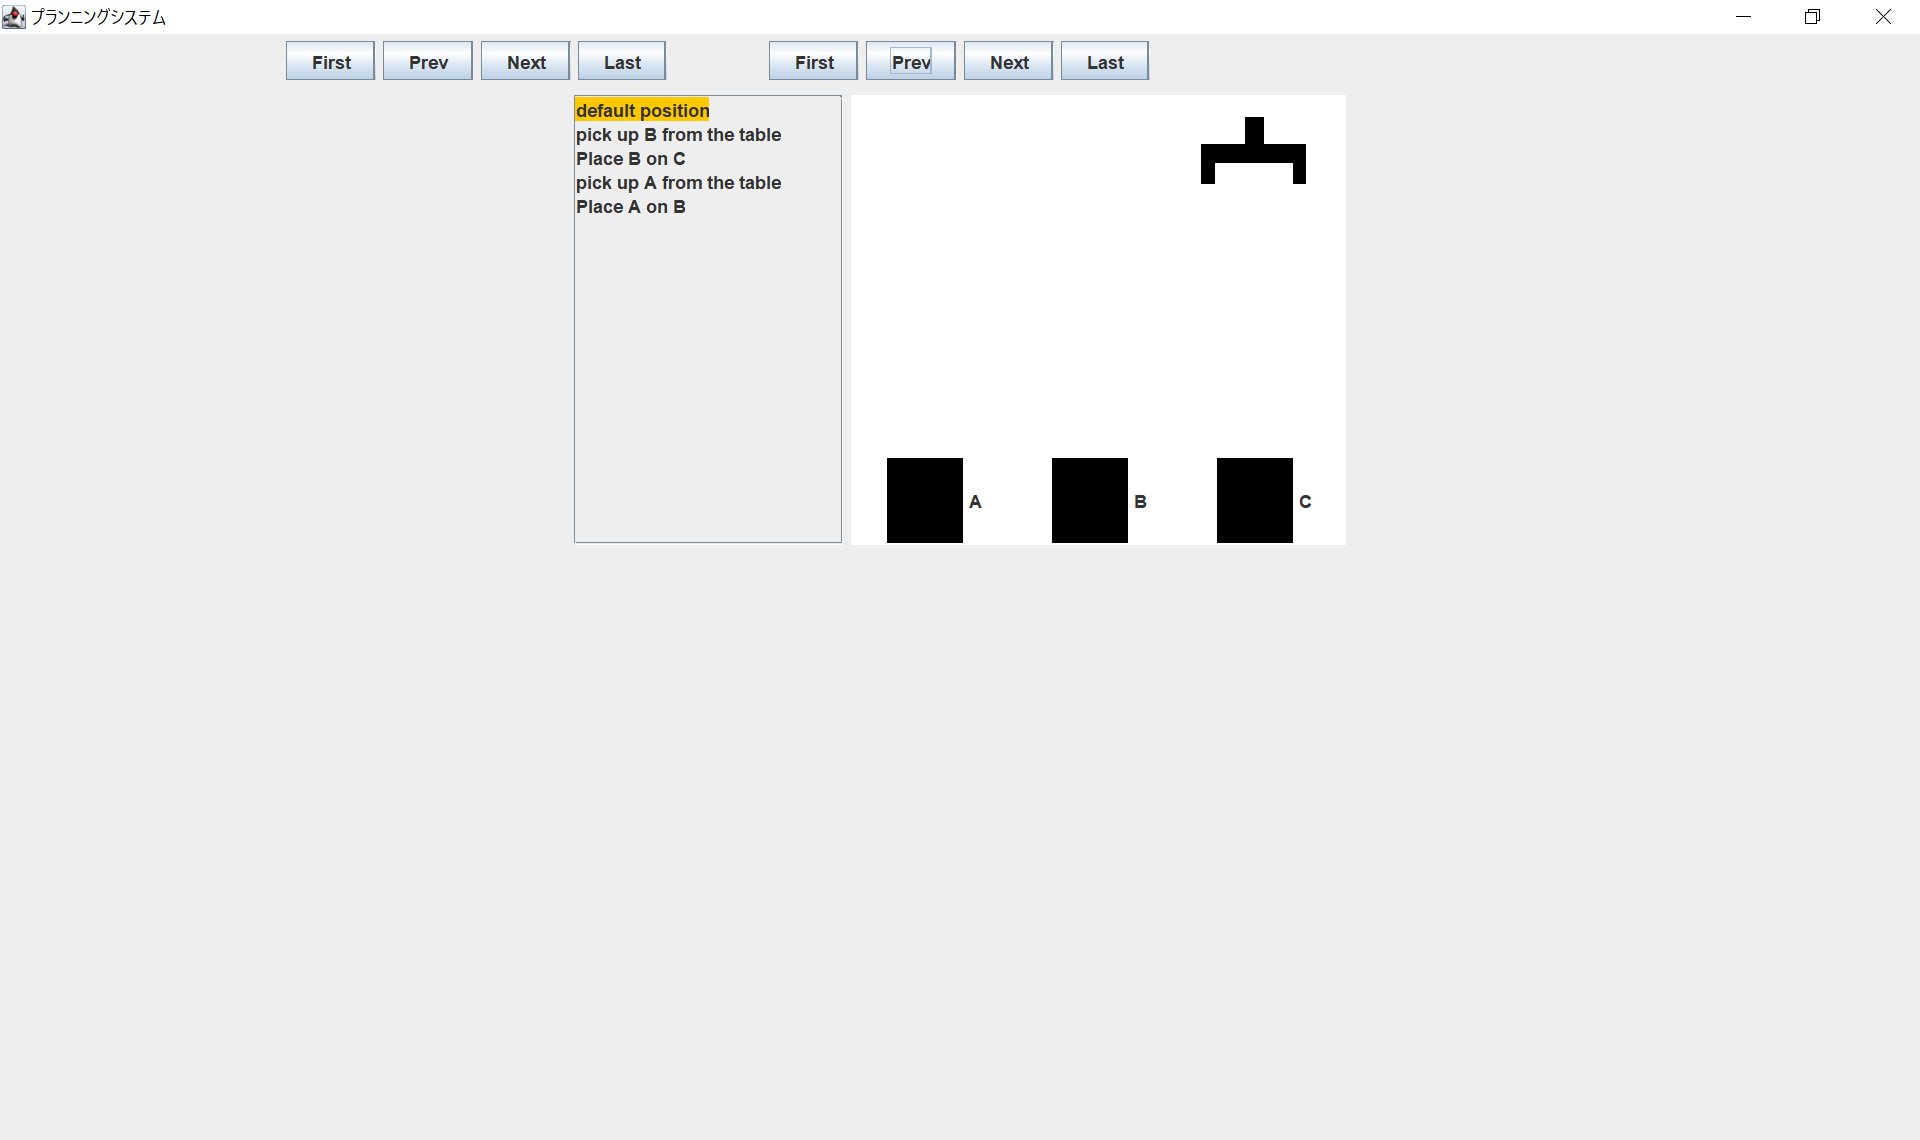
\includegraphics[scale=0.4]{images/ButErr.PNG}
    \caption{ウィンドウサイズを変更した際に起きるバグ}
    \label{fig:ButErr}
  \end{center}
\end{figure}
画像からも分かるように上に表示されるボタンの数が二重に表示されている.このときどちらのボタンも正しく動作を行うが,ウィンドウサイズの大きさによってはボタンが重なって表示されてしまうこともある.\\

\clearpage

これを改良した後の状態が,以下のようになる(図\ref{fig:ButOK}).\\

\begin{figure}[htbp]
  \begin{center}
    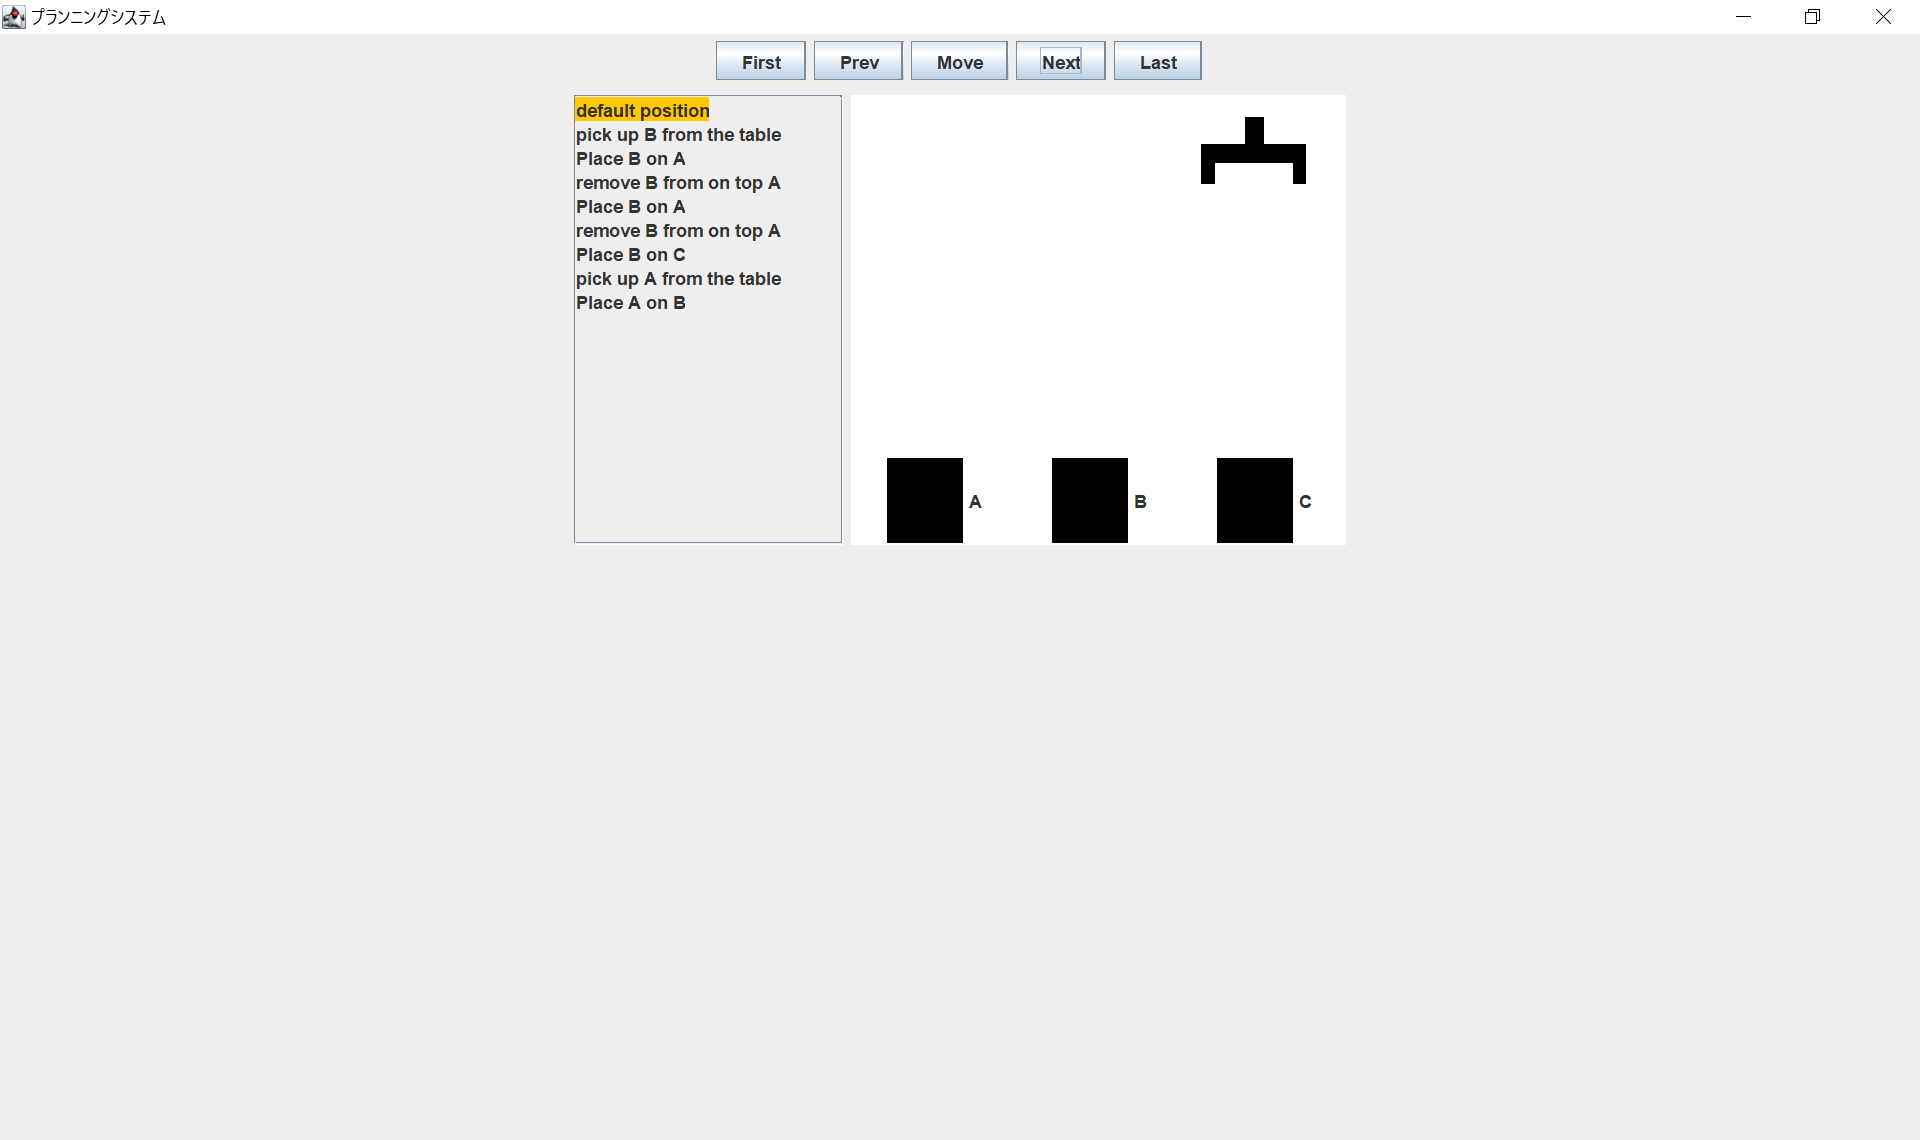
\includegraphics[scale=0.4]{images/ButOK.PNG}
    \caption{改良後のウィンドウ}
    \label{fig:ButOK}
  \end{center}
\end{figure}
ここからも分かるように,再描画後ウィンドウサイズを変更してもボタンが二重に表示されることが無くなった.\\
%\vspace{10mm}
\clearpage

次に,導出結果をより見やすくするためのMoveボタンの動作の実行結果を以下に示す.\\

実行した直後に現れる画面が以下のようになる(図\ref{fig:FirstPage}).\\

\begin{figure}[htbp]
  \begin{center}
    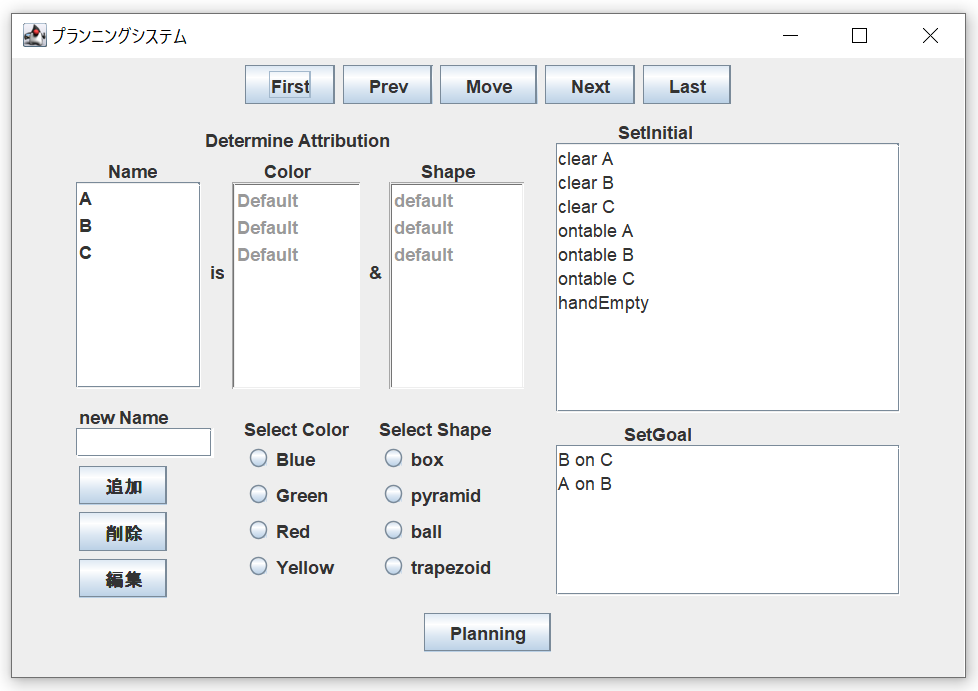
\includegraphics[scale=0.8]{images/FirstPage.PNG}
    \caption{Moveボタン追加後の初期画面}
    \label{fig:FirstPage}
  \end{center}
\end{figure}
前回の画面では,ウィンドウ上部にあるボタンが「First」「Prev」「Next」「Last」の四つであったが,今回の改良により新たに「Move」ボタンが追加されている.\\

\clearpage

Nextボタンを押すと,前回の課題同様に順に導出経路を確認することが出来る(図\ref{fig:Normal}).\\

\begin{figure}[htbp]
  \begin{center}
    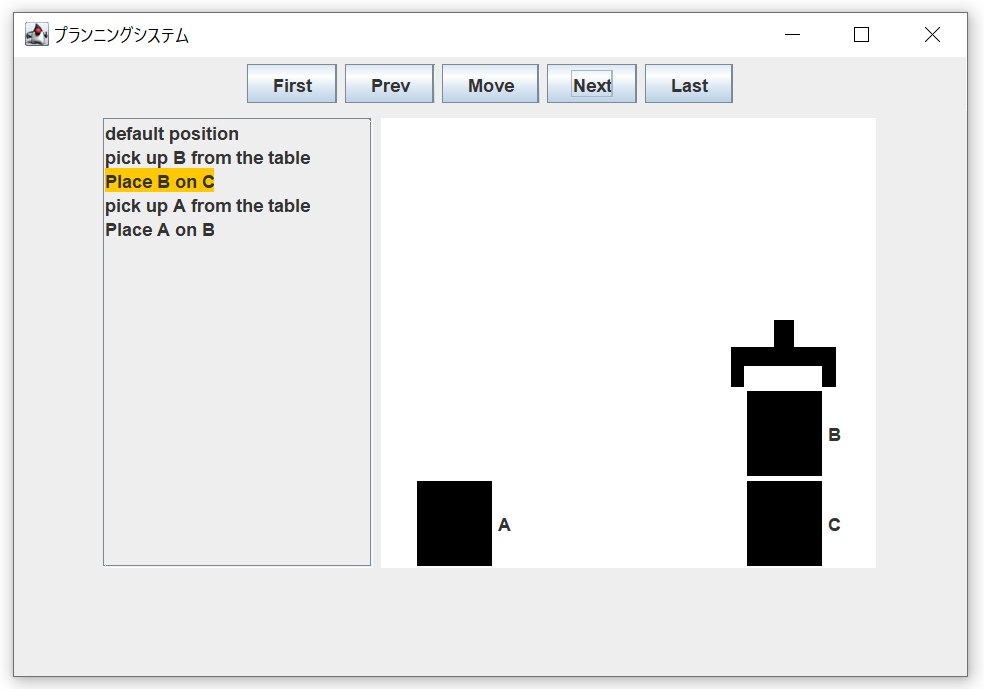
\includegraphics[scale=0.8]{images/Normal.PNG}
    \caption{Nextボタンで経路を確認するとき}
    \label{fig:Normal}
  \end{center}
\end{figure}
このとき,Nextボタンで状態が一つ進み,Prevボタンで状態が一つ戻る.またFirstボタンで初期画面に戻り,Lastボタンで最後の画面に遷移する.\par
これらの動作は前回作成したGUIと同じである.\\

\clearpage

Moveボタンを押した時の動作は以下のようになる(図\ref{fig:Move}).\\

\begin{figure}[htbp]
  \begin{center}
    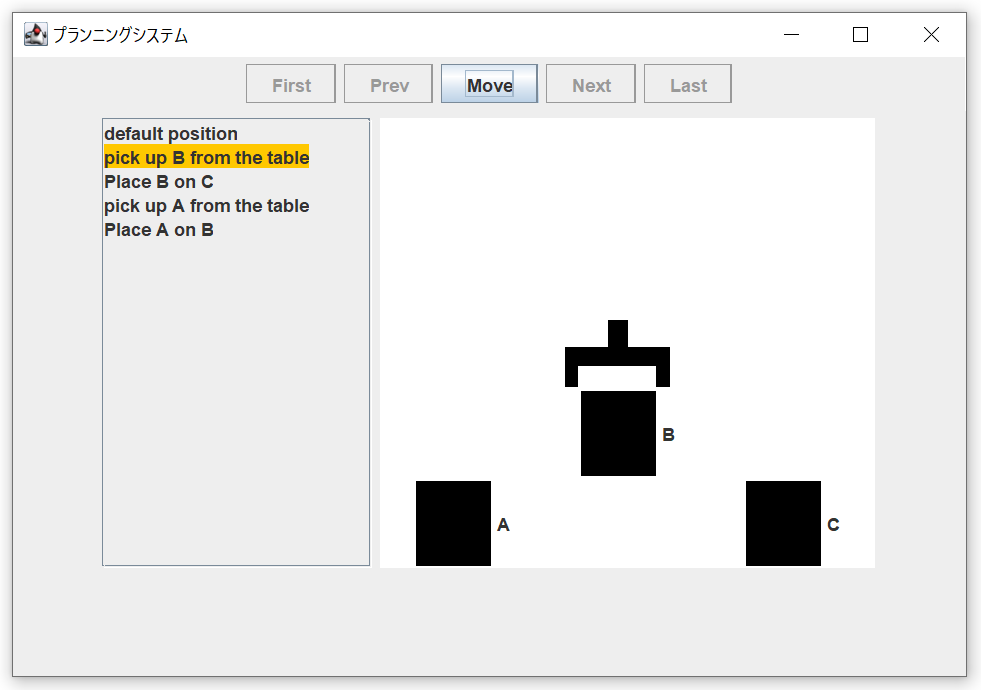
\includegraphics[scale=0.8]{images/Move.PNG}
    \caption{Nextボタンで経路を確認するとき}
    \label{fig:Move}
  \end{center}
\end{figure}
Moveボタンをクリックすると,その他のボタンが無効となり上図のようにクリック出来なくなる.さらにどの画面状態であっても初期状態の画面に遷移し,そこから一定時間ごとに導出経路が順に表示される.\par
最後に導出経路と使用したオペレータの出力画面が出力されると同時に無効になっていたボタンが有効になり,その他の操作が出来るようになる.

\clearpage
\subsection{考察}
今回の改良を行うにあたり実行結果を検証している際にGUIのウィンドウサイズを変えた際に起きてしまうバグを発見し,今回の課題としてまず改良を行った.\par
調べたところremoveAllメソッドを用いることでこの問題は解決できることが分かったが,このバグがなぜ起きるのかを調べたものの明確な答えを得ることが出来なかった.しかしこのバグが起きるのは再描画後であったため,再描画時に上書きする形で描画を行っていたことが原因ではないかと推測される.\par
前回課題ではウィンドウサイズの変更をしなくても良いGUIの作成を考えていたが,ユーザーがウィンドウサイズを変更する場合の可能性も考えてプログラムを作成する必要があると分かった.\\

さらに検証する中で,再描画時にウィンドウサイズを変更すると描画が一部消えてしまうことがあることも分かった.この場合も初めの描画時には消えることは無いため再描画に何か原因があると考えたが,これについては明確な原因とその対処方法が分からず,解決することが出来なかった.しかしマウスを近づけたりボタンをクリックすると消えた描画が元に戻るため,描画が出来ていないわけではないことは確認された.\par
この解決方法としては,再描画をしないようにプログラムを書き換える方法が考えられる.この場合私が使用しているCardLayoutでの状態遷移の描画を,再描画の際も以前のものを消さずにCardを増やす形にする方法が最も現実的であると考えた.しかしこの場合はNextボタンやPrevボタンでの処理が少し複雑になることや,繰り返しプランニングを行うことでCardの枚数が増え最終的にメモリ不足によるエラーが発生してしまうという欠点がある.そもそもGUIが再描画に適していないとも考えられたが今回の場合は描画自体は正しくできていることも考え,前回までの実装をそのまま採用した.\\

\clearpage

また以前の課題ではブロックが五つ以上ある場合は描画がGUIのウィンドウサイズを超えてしまい,ウィンドウサイズを大きくしなければ図が確認できなくなってしまうという問題があった.これを修正するため描画画面に対してスクロールバーをつけ,範囲を超えた描画を行う場合はスクロールバーを移動させ,ウィンドウサイズを変更することなく表示させることを考え実装を行った.\\

\vspace{10mm}

以下にその際のソースコードを示す(ソースコード\ref{scroll}).
\begin{lstlisting}[caption=スクロールバーの追加,label=scroll]
// 変数定義
JPanel card = new JPanel();
JPanel newpage = new JPanel();

// 画面を超えた描画時にスクロールバーにする
JScrollPane scrollpane = new JScrollPane();
// 最大描画サイズの指定
scrollpane.setPreferredSize(new Dimension(400, 350));
JViewport view = scrollpane.getViewport();
view.setView(newpage);
JPanel panel = new JPanel();
panel.add(scrollpane);
// パネルへの追加
card.add(splist);
card.add(panel);
\end{lstlisting}

この方法を用いることで,描画サイズが最大範囲を超えた時にはスクロールバーが追加されるようになった.

\clearpage

この時の実行結果が以下のようになる(図\ref{fig:tryScroll}).\\

\begin{figure}[htbp]
  \begin{center}
    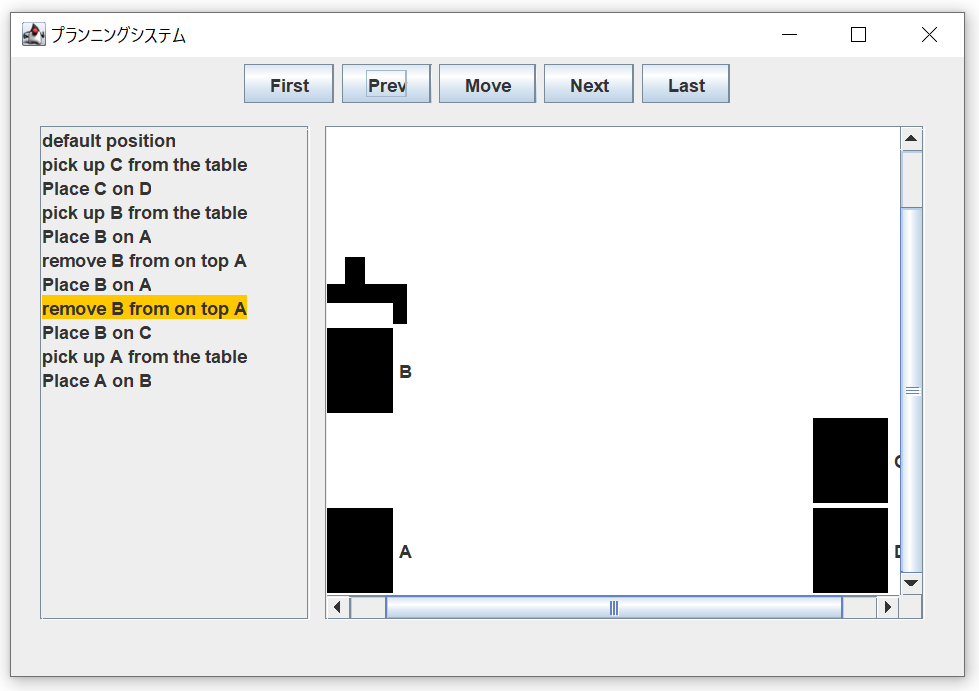
\includegraphics[scale=0.8]{images/tryScroll.PNG}
    \caption{スクロールバーを追加した場合}
    \label{fig:tryScroll}
  \end{center}
\end{figure}


ここから分かるように,スクロールバーを追加した場合描画サイズが表示可能サイズよりも大きいため,スクロールバーが出力された場合は一度にすべての状態を確認することが出来なくなってしまう.これでは現在の状態がどうなっているのか確認するのにいちいちスクロールバーを操作しなければならず,ブロックの数が増えれば増えるほど確認に大きな負担がかかる.\par
さらにスクロールバーは指定しなければ常に同じ位置にあるため,状況によってはその時動かしたブロックがスクロールバーを動かさなければ確認できない位置に存在する場合も考えられる.これではGUIとして使い難いことは明らかであるため,今回はスクロールバーの追加はしないこととした.\\

この解決方法としては,描画方法を変えることが最も効果的と考えられる.今回は描画にあらかじめ用意した画像を使用したが,この方法では表示する画像のサイズを変更することが出来ない.\par
直接描画を行う方法であればサイズの調節が可能になるため,ウィンドウサイズの変更をせず描画を行いたい場合は直接描画を行う方法が最良であると分かった.しかし前回の課題でも考察した通りその方法では座標設定を全て自身で行わなければならないため,座標管理が複雑になってしまうだけでなく,GUIの良さであるレイアウトマネージャーを活用出来なくなってしまう.このことから今回もこの方法での実装は行わないこととした.\\

\vspace{10mm}

Moveボタンの追加に関しては,動画のように滑らかな動きで経路を表現したいと考えたが,調べたところ滑らかな動きを実現するためにはレイアウトマネージャーを使用せずに座標で管理を行わなければならないことが分かった.前述の理由などから前回課題で作成したプログラムを活用して改良することを考え,今回は滑らかな動きをせず経路の過程を一回の操作(ボタンのクリック)で確認できるようにすることを目標とした.\\

導出経路の過程を表示するために用いたのがCardLayoutであったため,これを一定時間ごと次の画面に遷移させることで過程の表示が動的に行えると考えた.どの状態にあってもMoveボタンをクリックすれば初期状態から目標状態までの過程を表示できるようにするため,Moveボタンをクリックした段階でまず初期状態の画面に遷移し,そこから導出されている経路のCard枚数分だけ次のページへの遷移を繰り返す形とした.\par
このとき実行結果で述べたとおり他のボタンを動かせる状態にしておくと,Moveボタンによる繰り返しの回数と遷移状態がずれてしまうため表示がずれてしまう.そのため,Moveボタンで動作が行われている際はその他のボタンは無効にすることで正しい動作が行えるようにした.\\

%\vspace{10mm}

またこの機能を実装する中で,ボタンの操作検出による動作中は繰り返し作業や更なるボタンの操作を行うことが出来ないことが分かった.試行錯誤の中で,前回まではボタンのクリック操作をActionEventで検知していたが,MouseEventのmousePressedメソッドを用いればこれらの問題を解決できるのではないかと考え,mousePressedメソッドを使った実装を行った(ソースコード\ref{timer}参照).結果的にはMouseEventでも上記の動作は行うことが出来なかったため,その他の方法を調べ,タイマークラスを用いる方法を実装して求めている動作を実現させた.\par
結果的にはタイマークラスを用いることでMouseEventのmousePressedメソッドでなくActionEventでの実装でも同様の結果が得られることが分かったが,今回は様々な実装方法を学ぶという面からMouseEventを用いてプログラムを作成した.\par
GUIの場合も,同じ機能であっても様々な方法を用いて実装を行えることが分かった.



\section{必須課題6-1(発展課題5-5の改良)}
\begin{screen}
ブロックワールド内における物理的制約条件をルールとして表現せよ.
例えば,三角錐(pyramid)の上には他のブロックを乗せられない等,その世界における物理的な制約を実現せよ.
\end{screen}
\begin{screen}
    課題5にやり残した発展課題があれば参考にして拡張しても良いし,全く新しい独自仕様を考案しても構わない.
    自由に拡張するか,あるいはもし残っていた問題点があれば完成度を高めよ.
\end{screen}

\subsection{手法}
私は,前回課題の必須課題5-3と発展課題5-5を担当したので,今回の課題ではこれらに応用的な機能を付与することにした.
特に,課題5-5で実装した「禁止制約」機能を拡張し,新たにルールの挿入/削除/編集機能を追加することとした.
また,私の担当範囲は内部処理に留まるため,前回作成した属性クラスAttributions内へのメソッド追加とPresenterクラスからの利用までを担当とする.

% \begin{figure}[!hbt]
%   \centering
%   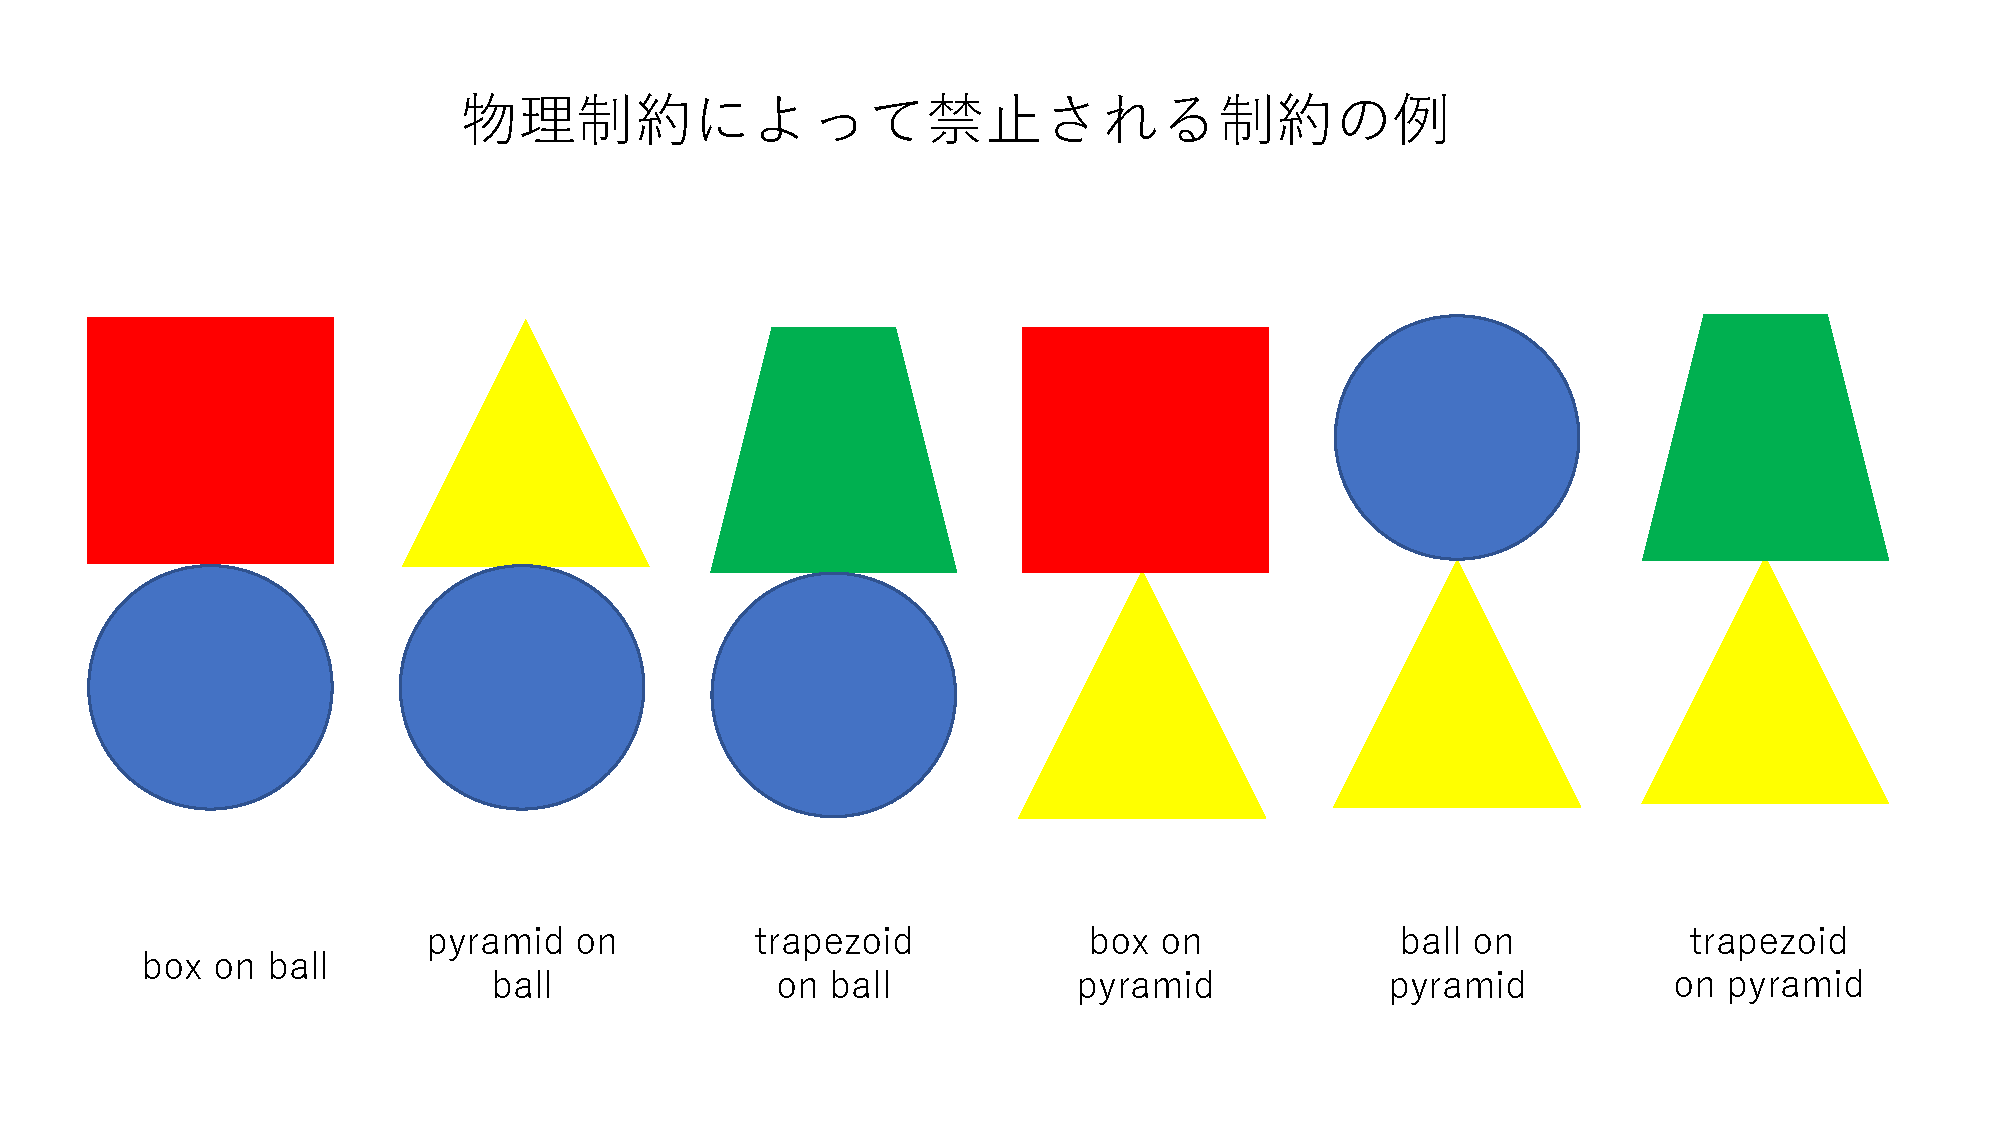
\includegraphics[scale=0.35]{images/prohibit-rules.pdf}
%   \caption{物理制約によって禁止される制約の例}
% \end{figure}

\subsection{実装}
まず,Attributionsクラス内部に,禁止制約への新たなルールの挿入/削除/編集を行う以下のメソッドを追加した.
\begin{description}
\item[insertProhibitRules(ArrayList \textless String\textgreater targetRules)] 新たなルールを挿入するメソッド
\item[deleteProhibitRules(ArrayList \textless String\textgreater targetRules)] 指定したルールを削除するメソッド
\item[editProhibitRules(String beforeRule, String afterRule)] 指定したルールを編集するメソッド
\end{description}
以下に各メソッドについてソースコードと説明を示す.

はじめに,新たなルールを挿入するメソッドを示す.
\begin{lstlisting}[caption=insertProhibitRulesメソッドの実装, label=mid]
    public void insertProhibitRules(ArrayList<String> targetRules) {
		prohibitRules.addAll(targetRules);
		prohibitBlockStates.clear();
		prohibitBlockStates = editStatementList(prohibitRules);
	}
\end{lstlisting}
まず,挿入する対象のルールリストを引数で受け取り,2行目で既存の禁止制約リストに全て加える.
さらに,3行目ではブロック名による禁止制約リストを一度全て削除し,更新されたルールリストを元にして,4行目で作成し直している. \\

次に,指定されたルールを削除するメソッドを示す.
\begin{lstlisting}[caption=deleteProhibitRulesメソッドの実装, label=mid]
    public void deleteProhibitRules(ArrayList<String> targetRules) {
		for(String targetRule: targetRules) {
			prohibitRules.remove(targetRule);
		}
		prohibitBlockStates.clear();
		prohibitBlockStates = editStatementList(prohibitRules);
	}
\end{lstlisting}
まず,削除する対象のルールリストを引数で受け取り,2~4行目で既存の禁止制約リストから削除する処理を行なっている.
5,6行目では先ほど同様にブロック名による表現に反映している. \\

続いて,指定されたルールを編集するメソッドを示す.
\begin{lstlisting}[caption=editProhibitRulesメソッドの実装, label=mid]
    public void editProhibitRules(String beforeRule, String afterRule) {
		prohibitRules.remove(beforeRule);
		prohibitRules.add(afterRule);
		prohibitBlockStates.clear();
		prohibitBlockStates = editStatementList(prohibitRules);
	}
\end{lstlisting}
まず,編集する対象のルールリストを引数で受け取り,2行目で既存の禁止制約リストから編集前ルールを削除し,3行目で編集後ルールを挿入する処理を行なっている.
4,5行目では先ほど同様にブロック名による表現に反映している. \\

また,Presenterクラスにおいてもこれらを利用する同名メソッドを定義した. \\
なお,これらのメソッドでは,引数で受け取るリストの要素数によって,GUIへの反映処理を切り分けられる実装となっている.
具体的には,要素数が0の場合やnullといった場合には,処理を行うことができないように,GUIへとフィードバックを行うように変更した.

\subsection{実行例}
以下に,今回追加したメソッドをテストした結果を示す.
\begin{lstlisting}[caption=editProhibitRulesメソッドの実装, label=mid]
    ~/Programming2/individual_report/attributions
    ●java Test   
    **** Attribution rules ****
    A is blue
    A is ball
    B is green
    B is trapezoid
    C is red
    C is box
    ###### Add prohibitRule ######
    ****** ProhibitRule:ball on ball ******
    ****** ProhibitRule:trapezoid on ball ******
    ****** ProhibitRule:trapezoid on trapezoid ******
    ****** ProhibitRule:box on ball ******
    ****** ProhibitRule:box on box ******
    ****** ProhibitRule:pyramid on ball ******
    ****** ProhibitRule:ball on pyramid ******
    ****** ProhibitRule:box on pyramid ******
    ****** ProhibitRule:trapezoid on pyramid ******
    ****** ProhibitRule:pyramid on pyramid ******
    ++++++ EditStatement ++++++
    ball on ball =====> A on A
    trapezoid on ball =====> B on A
    trapezoid on trapezoid =====> B on B
    box on ball =====> C on A
    box on box =====> C on C
    pyramid on ball =====> pyramid on A
    ball on pyramid =====> A on pyramid
    box on pyramid =====> C on pyramid
    trapezoid on pyramid =====> B on pyramid
    pyramid on pyramid =====> pyramid on pyramid
    
    ----- insert rules -----
    blue on red
    green on blue
    ++++++ EditStatement ++++++
    ball on ball =====> A on A
    trapezoid on ball =====> B on A
    trapezoid on trapezoid =====> B on B
    box on ball =====> C on A
    box on box =====> C on C
    pyramid on ball =====> pyramid on A
    ball on pyramid =====> A on pyramid
    box on pyramid =====> C on pyramid
    trapezoid on pyramid =====> B on pyramid
    pyramid on pyramid =====> pyramid on pyramid
    blue on red =====> A on C
    green on blue =====> B on A
    
    ----- delete rules -----
    blue on red
    ++++++ EditStatement ++++++
    ball on ball =====> A on A
    trapezoid on ball =====> B on A
    trapezoid on trapezoid =====> B on B
    box on ball =====> C on A
    box on box =====> C on C
    pyramid on ball =====> pyramid on A
    ball on pyramid =====> A on pyramid
    box on pyramid =====> C on pyramid
    trapezoid on pyramid =====> B on pyramid
    pyramid on pyramid =====> pyramid on pyramid
    green on blue =====> B on A
    
    変更前のルール:green on blue
    変更後のルール:yellow on blue
    ++++++ EditStatement ++++++
    ball on ball =====> A on A
    trapezoid on ball =====> B on A
    trapezoid on trapezoid =====> B on B
    box on ball =====> C on A
    box on box =====> C on C
    pyramid on ball =====> pyramid on A
    ball on pyramid =====> A on pyramid
    box on pyramid =====> C on pyramid
    trapezoid on pyramid =====> B on pyramid
    pyramid on pyramid =====> pyramid on pyramid
    yellow on blue =====> yellow on A
\end{lstlisting}

3~31行目で属性ルールおよび禁止制約の追加と,禁止制約をブロック名による表現に変換する処理の結果を示している.
ここまでは,前回課題での実装範囲と同じである. \\

33~48行目においては,禁止制約挿入処理とブロック名での表現への変換処理の結果を示している.
特に注目すべきは,47・48行目で,これらは新たに挿入された禁止制約の影響を受けた部分である.
先ほどは存在しなかった
\begin{verbatim}
    blue on red=====>A on C
    green on blue=====>B on A
\end{verbatim}
という表現が現れている. \\

50~63行目においては,禁止制約削除処理とブロック名での表現への変換処理の結果を示している.
特に注目すべきは,62行目と63行目の間で,先ほどは存在した
\begin{verbatim}
    blue on red=====>A on C
\end{verbatim}
が削除されてなくなっている.

65~78行目においては,禁止制約編集処理とブロック名での表現への変換処理の結果を示している.
特に注目すべきは,78行目で,先ほどは
\begin{verbatim}
    green on blue=====>B on A
\end{verbatim}
となっていた部分が,
\begin{verbatim}
    yellow on blue=====>yellow on A
\end{verbatim}
として編集されている.

\subsection{考察}
今回,禁止制約を自由に挿入/削除/編集することができる機能を追加したことによって,
前回課題では物理法則に則ったもののみであったが,ユーザー独自のカスタマイズを行うことが可能となった.
特に,色などの属性による制約を加えることによって,さらに複雑な問題設定が可能となる. \\
プランニングなど,知識ベース型の人工知能システムは,十分な知識を取得可能な場面においては,
データ駆動型のシステムに比べて低コストで高精度の予測を行えることもあり,現在でも非常に有効な手段である.
むしろ,このような場合には,知識ベース型のシステムを選択すべきであり,いたずらにデータ駆動型の機械学習を導入すべきではないとも考えられる. \\
双方の特徴を知り,長所・短所を正しく認識した上で社会への応用が可能となることを胸に刻む必要があると感じた.
また,ただ理論やアルゴリズムを組み上げるのみでは十分ではなく,「多くの人に使ってもらえるようなUI/UX」を考える必要もある.
情報プロダクトにおいても,エンジニアの自己満足ではなくユーザーの側に立ってプロダクトを作ることができて初めて社会的価値があると言える. \\
さらに,本演習前半の「Javaによる知識システム実装」では,知識システムプログラムの改良とGUI実装を行なうことを通して,
グループワークの難しさも体験した.
個人それぞれの事情や性格が違うので,なかなか上手くまとまらない場面もあり,毎回レポートやプログラムの完成が提出期限間際となっていた.
私個人としては,早めに課題を終わらせておく性格であるため,そうでない人と協調して作業を行うことは非常に難しく感じた.
しかし,GUIなど特定の個人が興味を抱いている分野に関しては率先して取り組む姿が見られ,担当者に頼もしさを感じることもあった.
実際に社会に出た際に求められるスキルとして,グループ開発は必須となってくると考えられるので,現段階から少しでもそれを体験できたのは非常に良かったと感じている.



\section{必須課題6-1(発展課題5-7の改良)}
\begin{screen}
3次元空間 (実世界) の物理的な挙動を考慮したブロックワールドにおけるプランニングを実現せよ.
なお,物理エンジン等を利用する場合,Java以外の言語のフレームワークを使って実現しても構わない.
\end{screen}
\begin{screen}
課題5にやり残した発展課題があれば参考にして拡張しても良いし,全く新しい独自仕様を考案しても構わない.自由に拡張するか,あるいはもし残っていた問題点があれば完成度を高めよ.
\end{screen}
私の担当箇所は,発展課題5-7に対してUnityを用いて実装したプログラムの,GUI改善やプランニングへの機能追加である.

\subsection{手法}
発展課題5-7では,ブロックワールドにおけるプランニングを実現するための過程として,以下のような実装を行った.
\begin{enumerate}
\item 空間やプランに関するオブジェクトの生成.
\item プランニングを行うための,オブジェクトの動作等に関するスクリプトの作成.
\end{enumerate}

これに引き続いて今回は,ブロックワールドにおけるプランニングを実現するために,以下のような方針を立てた.
\begin{enumerate}
\item プランに用いるブロックをより正確に生成できるようにする.
\item ブロックの管理を容易にする.
\item プランニングの情報を可視化する.
\end{enumerate}

1.に関して,GUIを画面上に表示することで,ブロックを名前や色,形を指定した上で生成できるような仕様とした.

2.に関して,オブジェクトの情報を一覧で表示して生成したオブジェクトの管理を視覚的に行えるような仕様とした.また,フォーカスしているブロックを視覚的に確認できるように,選択中のオブジェクトのアウトラインが表示されるような仕様とした.

3.に関して,2.で作成する一覧と連動して,選択したブロックの情報が画面左下のステータスバーで確認できるようにした.

\subsection{実装}
発展課題5-7で作ったオブジェクトは以下のとおりである.
\begin{description}
\item[Main Camera] 主カメラに関するオブジェクト.Room全体をやや見下ろし気味に映す.
\item[Directional Light] オブジェクト全体を照らす照明.
\item[Master] スクリプトをアタッチするための空オブジェクト.
\item[Room] 6個のPlaneオブジェクトを子に持つ,立方体の部屋を構成するオブジェクト.
\item[Cube] 直方体のブロックを生成するプレハブ.
\item[Sphere] 球のブロックを生成するプレハブ.
\item[Torus] 円環体のブロックを生成するプレハブ.
\end{description} 

新しく作った主なオブジェクトは以下のとおりである.
\begin{description}
\item[EventSystem] GUIにおいてButtonやInputFieldを機能させるための,フォーカス情報等を掌るオブジェクト.
\item[Canvas] Generator,Preparator,Staterを子オブジェクトに持つ,GUIの大元となるオブジェクト.
\item[Generator] オブジェクトを生成するためのパネル.子オブジェクトにInputFieldName,DropdownColor,DropdownShape,ButtonGenを持つ.
\item[Preparator] 生成したオブジェクトの一覧を管理するパネル.子オブジェクトにScrollView,ButtonRm,ButtonPlanningを持つ.
\item[Stater] オブジェクトの情報等を表示するためのパネル.子オブジェクトにTextStatus,Scrollbarを持つ.
\item[ListObj] PreparatorにおけるScrollViewの要素となるプレハブ.
\end{description} 

C\#スクリプトでは以下のものが実装されている.
\begin{description}
\item[Clicked] クリックされたオブジェクトにフォーカスを当てるスクリプト.Masterにアタッチされる.
\item[Operationg] Clickedでフォーカスされたオブジェクトにキーボード入力を反映するスクリプト.Masterにアタッチされる.
\item[Generator] Generatorオブジェクトで得た情報に合わせて,ブロックを生成するスクリプト.ButtonGenにアタッチされる.
\item[Destroyer] Preparatorオブジェクトで選択されたブロックを削除するためのスクリプト.ButtonRmにアタッチされる.
\item[Manager] ListObjプレハブにアタッチされる,各インスタンスが1対1で対応するブロックを保持するためのスクリプト.
\item[SelectOnList] ListObjプレハブにアタッチされる,インスタンスが自身にアウトラインや削除のフォーカスを当てるためのスクリプト.
\item[Starter] GUIの一部を非表示にし,プランニングを開始するためのスクリプト.ButtonPlanningにアタッチされる.
\item[CollisionGetter] 自身と衝突中のブロックを保持するスクリプト.各ブロックにアタッチされる.
\item[StateGetter] SelectOnListでフォーカスされたブロックと衝突中のブロックをStaterに表示するスクリプト.Masterにアタッチされる.
\end{description}

\subsubsection{プランに用いるオブジェクトをより正確に生成できるようにする.}
Unity\cite{unity}においてGUIを作成するために,Unityの標準機能に含まれるuGUI\cite{ugui}を用いた.

まず,GUI制作をUnity上で開始するために,Canvasオブジェクトを生成した.Canvasオブジェクトは実行環境によって,そのサイズが動的に変化するため,シーンビューにおける大きさは意味を持たない.その仕様を理解するまでは扱いに戸惑った.

次に,ブロック生成のためのGUIであるGeneratorオブジェクト(図\ref{fig:an1})を作るために,GeneratorオブジェクトにはPanelを,名前を入力するためのフォーム(InputFieldName)にはInputFieldを,色や形の選択(DropdownColor,DropdownShape)にはDropdownを,生成ボタン(ButtonGen)にはButtonをそれぞれ用いた.これらUIに関するパーツはいずれもRectTransformコンポーネントを用いて配置される.

RectTransformの特徴として,アンカーとピボットが挙げられる.これらはブロック等のオブジェクトの座標指定で用いられるTransformコンポーネントには含まれない.今回ピボットは用いなかったが,アンカーはGUIパーツの配置を行う上では欠かせないものであることが分かった.

アンカーは,指定した位置を基準として,オブジェクトの相対座標を指定するものである.図\ref{fig:an1}に示すように,Canvasの右上部である位置に表示されている4つの三角がアンカーの基準点を示すものであり,パネルはアンカーから左下部に相対座標で配置されている.これにより,実行環境により画面サイズが変化しても,図\ref{fig:an2}や図\ref{fig:an3}で示すようにレイアウトを崩さずに表示されることが確認できる.

\begin{figure}[!hbt]
  \begin{center}
    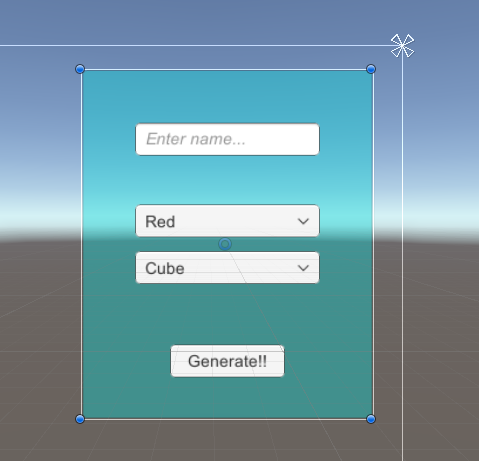
\includegraphics[scale=0.5]{images/BWP_Work6/anchor1.png}
  \end{center}
  \caption{Generatorオブジェクト}
  \label{fig:an1}
\end{figure}

\begin{figure}[!hbt]
  \begin{center}
    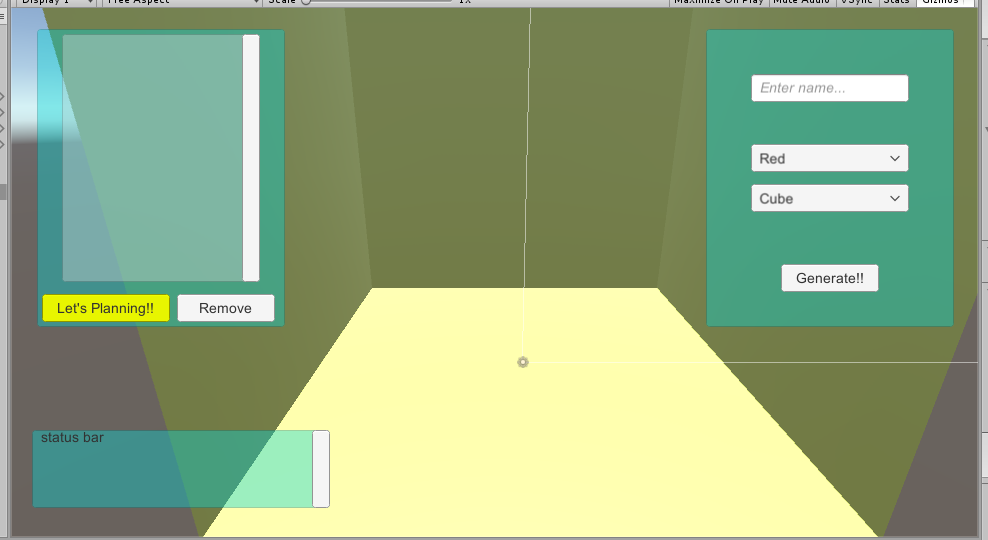
\includegraphics[scale=0.5]{images/BWP_Work6/anchor2.png}
  \end{center}
  \caption{横長の画面における表示}
  \label{fig:an2}
\end{figure}

\begin{figure}[!hbt]
  \begin{center}
    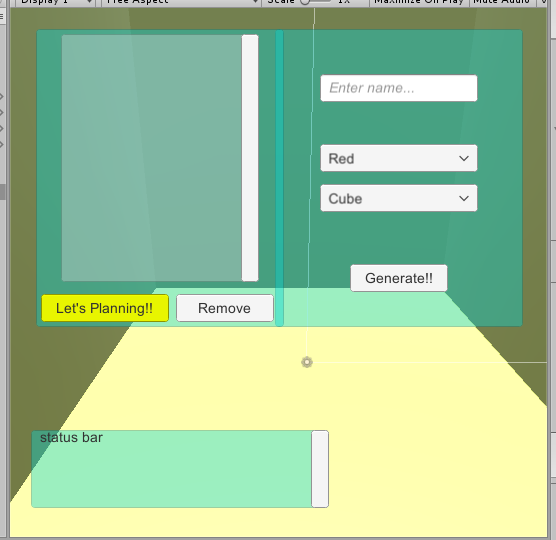
\includegraphics[scale=0.5]{images/BWP_Work6/anchor3.png}
  \end{center}
  \caption{縦長の画面における表示}
  \label{fig:an3}
\end{figure}

\clearpage

次に,配置したGenerator内のオブジェクトを用いて,ブロックを生成するためのスクリプト(Generator.cs)を生成する.
ブロックはソースコード\ref{src:gen}で示すように生成される.

\begin{lstlisting}[caption=Generatorクラス, label=src:gen]
public class Generator : MonoBehaviour
{
    ...
    public void Generate()
    {
        ...
        GameObject obj = (GameObject)Resources.Load("Cube");
        switch (ddShape.value)
        {
            case 0:
                obj = (GameObject)Resources.Load("Cube");
                break;
            case 1:
                obj = (GameObject)Resources.Load("Sphere");
                break;
            case 2:
                obj = (GameObject)Resources.Load("Torus");
                break;
        }
        GameObject target = Instantiate(obj, obj.transform.position, Quaternion.identity);
        target.name = name;
        target.GetComponent<Renderer>().material.color = getColor(ddColor.value).color;

        GameObject _text = Instantiate(textPrefab, content.transform);
        _text.GetComponentInChildren<Text>().text = name;
        _text.GetComponent<Manager>().planObj = target;
    }
    
    ...

    Material getColor(int num)
    {
        Material color = matR;
        switch(num)
        {
            case 0:
                color = matR;
                break;
            case 1:
                color = matG;
                break;
            case 2:
                color = matB;
                break;
        }
        return color;
    }
}
\end{lstlisting}

ddShape.valueを介してDropdownShapeで選択された形を選択し,Resource.Loadメソッドでプレハブを取得している.取得したプレハブをInstantiateメソッドで生成し,生成したインスタンスの名前をInputFieldNameで入力した名前に書き換え,色をddColor.valueを介してDropdownShapeで選択された色に書き換えている.

このスクリプトをButtonGenにアタッチすることで,ボタンをクリックしたときにこのスクリプトは呼び出され,実行される.
\clearpage

\subsubsection{ブロックの管理を容易にする.}
ブロックを管理するためのGUIであるPreparatorオブジェクト(図\ref{fig:pre})を作るために,PreparatorオブジェクトにはPanelを,ブロックを表示するリスト(ScrollView)にはScrollViewを,リスト内の要素(ListObj)にはButtonをプレハブ化したもの,リスト内の要素削除ボタン(ButtonRm)とプランニング開始ボタン(ButtonPlanning)にはButtonをそれぞれ用いた.

\begin{figure}[!hbt]
  \begin{center}
    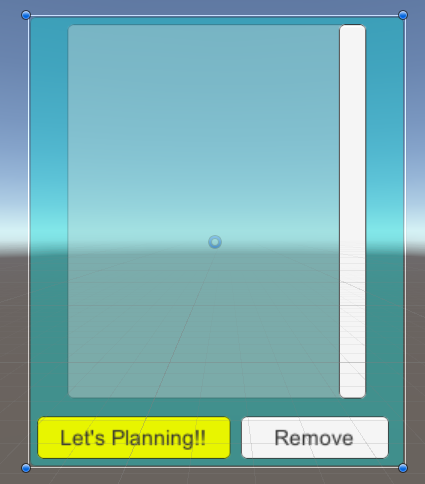
\includegraphics[scale=0.5]{images/BWP_Work6/preparator.png}
  \end{center}
  \caption{Preparatorオブジェクト}
  \label{fig:pre}
\end{figure}

ScrollViewを作成する\cite{sv}にあたり,ListObjは要素の選択を可能にするために,Buttonを用いて実装した.

Generatorスクリプト(ソースコード\ref{src:gen})の変数\_textによって,ListObjからインスタンスが生成されている.この際,スクロールバーに表示するためには適切な位置の子オブジェクトとして格納する必要がある.これは,Instantiateの引数に親オブジェクトのtransformを渡すことで実現した.
また,ここで生成したインスタンスに,先程生成したブロックのインスタンスへの参照も,Managerスクリプトの変数を介して渡している.これにより,ListObjのインスタンスから対応するブロックへのアクセスを可能としている. \\

次に,ScrollViewから選択した要素にアウトラインを付けるためのスクリプトSelectOnList,StateGetterを実装する.

まず,アウトラインはUnityの標準機能に備わっていないため,アセットQuickOutline\cite{outline}を導入し,各ブロックに非アクティブ状態でアタッチした.

その上で,引数で渡されたブロックのアウトラインをアクティブにするStateGetterクラス内のFocusOutlineメソッドを,ソースコード\ref{src:outline}に示す.

\begin{lstlisting}[caption=StateGetterクラス内のFocusOutlineメソッド, label=src:outline]
    public GameObject target;
    
    public void FocusOutline (GameObject newObj) {
        if (target != null) {
            target.GetComponent<Outline> ().enabled = false;
        }
        if (newObj != null) {
            newObj.GetComponent<Outline> ().enabled = true;
        }
        target = newObj;
    }
\end{lstlisting}

アウトラインをアクティブにしたブロックをtargetに保持することで,フォーカスが外れた際の非アクティブ化も同時に行えるようになっている.StateGetterはMasterに1つだけアタッチされることで,フォーカスの管理を一元的に行うことを可能とした.

SelectOnListスクリプトは各ListObjインスタンスにアタッチされることで,フォーカスが当てられたときにSelectOnListスクリプトからFocusOutlineメソッドを呼び出すことで,自身にアウトラインを付けることができる.(図\ref{fig:off},\ref{fig:on})

\begin{figure}[!hbt]
  \begin{center}
    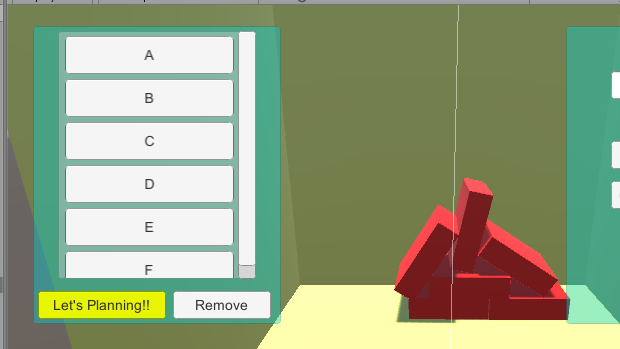
\includegraphics[scale=0.5]{images/BWP_Work6/outline1.png}
  \end{center}
  \caption{非フォーカス時}
  \label{fig:off}
\end{figure}

\begin{figure}[!hbt]
  \begin{center}
    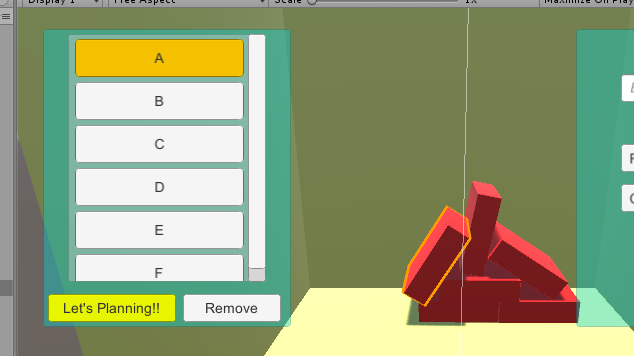
\includegraphics[scale=0.5]{images/BWP_Work6/outline2.png}
  \end{center}
  \caption{フォーカス時}
  \label{fig:on}
\end{figure}
\clearpage

\subsubsection{プランニングの情報を可視化する.}
プランニングの情報表示のためのGUIであるStaterオブジェクト(図\ref{fig:stater})を作るために,StaterオブジェクトにはPanelを,情報を表示するテキスト(TextStatus)にTextを用い,一度に全部を表示できないときのためにScrollbarを作成した\cite{sb}.

\begin{figure}[!hbt]
  \begin{center}
    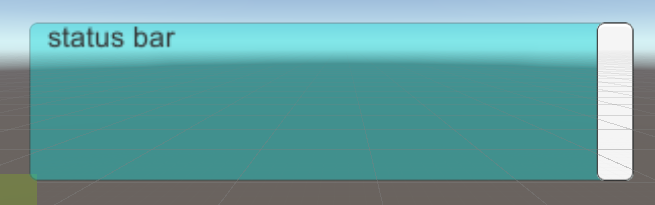
\includegraphics[scale=0.5]{images/BWP_Work6/stater.png}
  \end{center}
  \caption{Staterオブジェクト}
  \label{fig:stater}
\end{figure}

フォーカスされたオブジェクトの衝突情報を取得するために,CollisionGetterスクリプトを作成し,各ブロックにアタッチした.それをソースコード\ref{src:collision}に示す.

\begin{lstlisting}[caption=CollisionGetterクラス, label=src:collision]
public class CollisionGetter : MonoBehaviour {

    public List<GameObject> colList;

    void Awake () {
        colList = new List<GameObject> ();
    }

    void OnCollisionStay (Collision collision) {
        if (!colList.Contains(collision.gameObject)) {
            colList.Add (collision.gameObject);
        }
    }
    void OnCollisionExit (Collision collision) {
        colList.Remove (collision.gameObject);
    }
}
\end{lstlisting}

衝突相手のブロック名がcolListに1つだけ格納される.この際,同じブロックに対して複数の衝突判定を持つときにcolListに複数同じ要素が含まれないようにするために,要素の追加はOnCollisionEnterメソッドではなくOnCollisionStayメソッドを用いて常に監視することで,colListの要素が常に正確になるような実装をした.

このリストをStateGetterから取得し,Staterに反映することで,フォーカスしたブロックの衝突判定を,常に可視化することを実現した.

\subsection{実行例}
task5-7/build/Block World Planning.exeを起動したところ,図\ref{fig:run0}のような画面が得られる.

\begin{figure}[!hbt]
  	\begin{center}
  		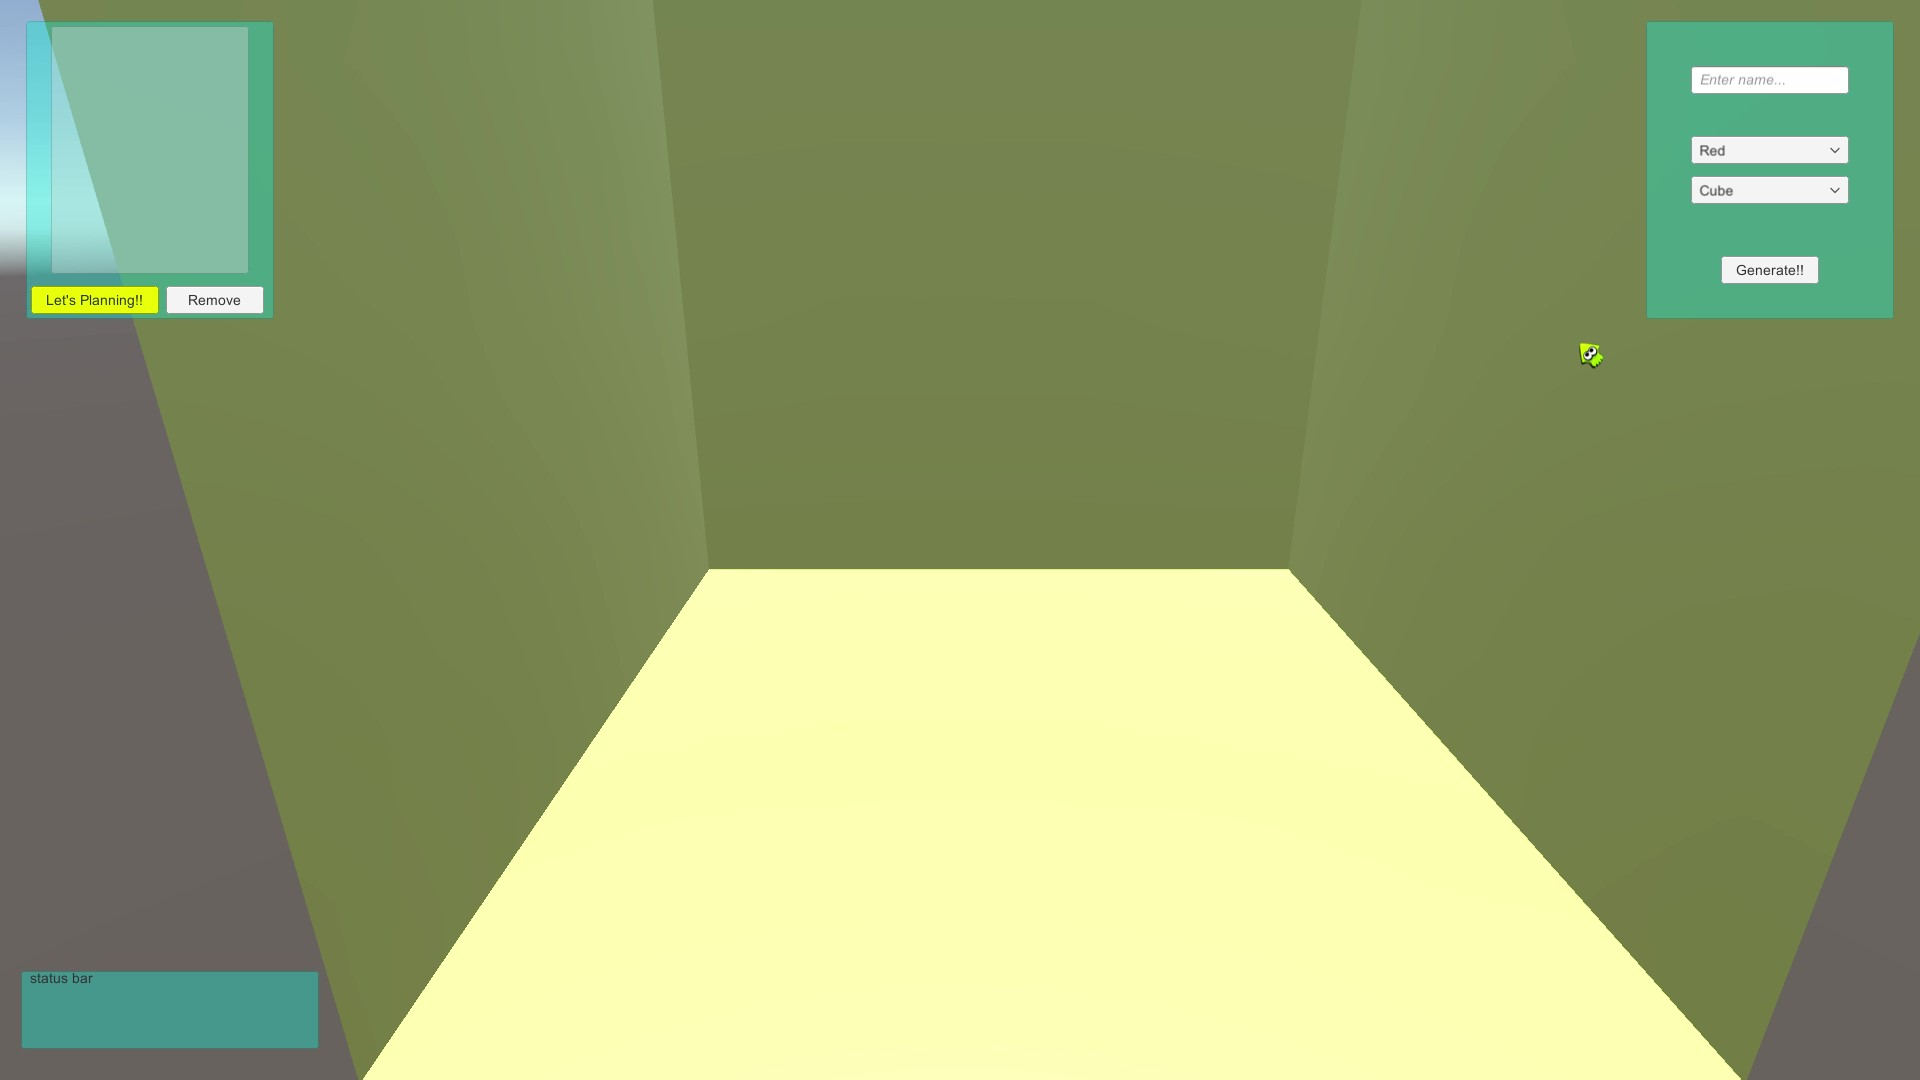
\includegraphics[scale=0.2]{images/BWP_Work6/bwp0.jpg}
	\end{center}
  	\caption{起動時の画面}
  	\label{fig:run0}
\end{figure}
\clearpage

Generatorを用いてブロックを生成すると,Preparatorにも反映されることが分かる(図\ref{fig:run1},\ref{fig:run2}).

\begin{figure}[!hbt]
  	\begin{center}
  		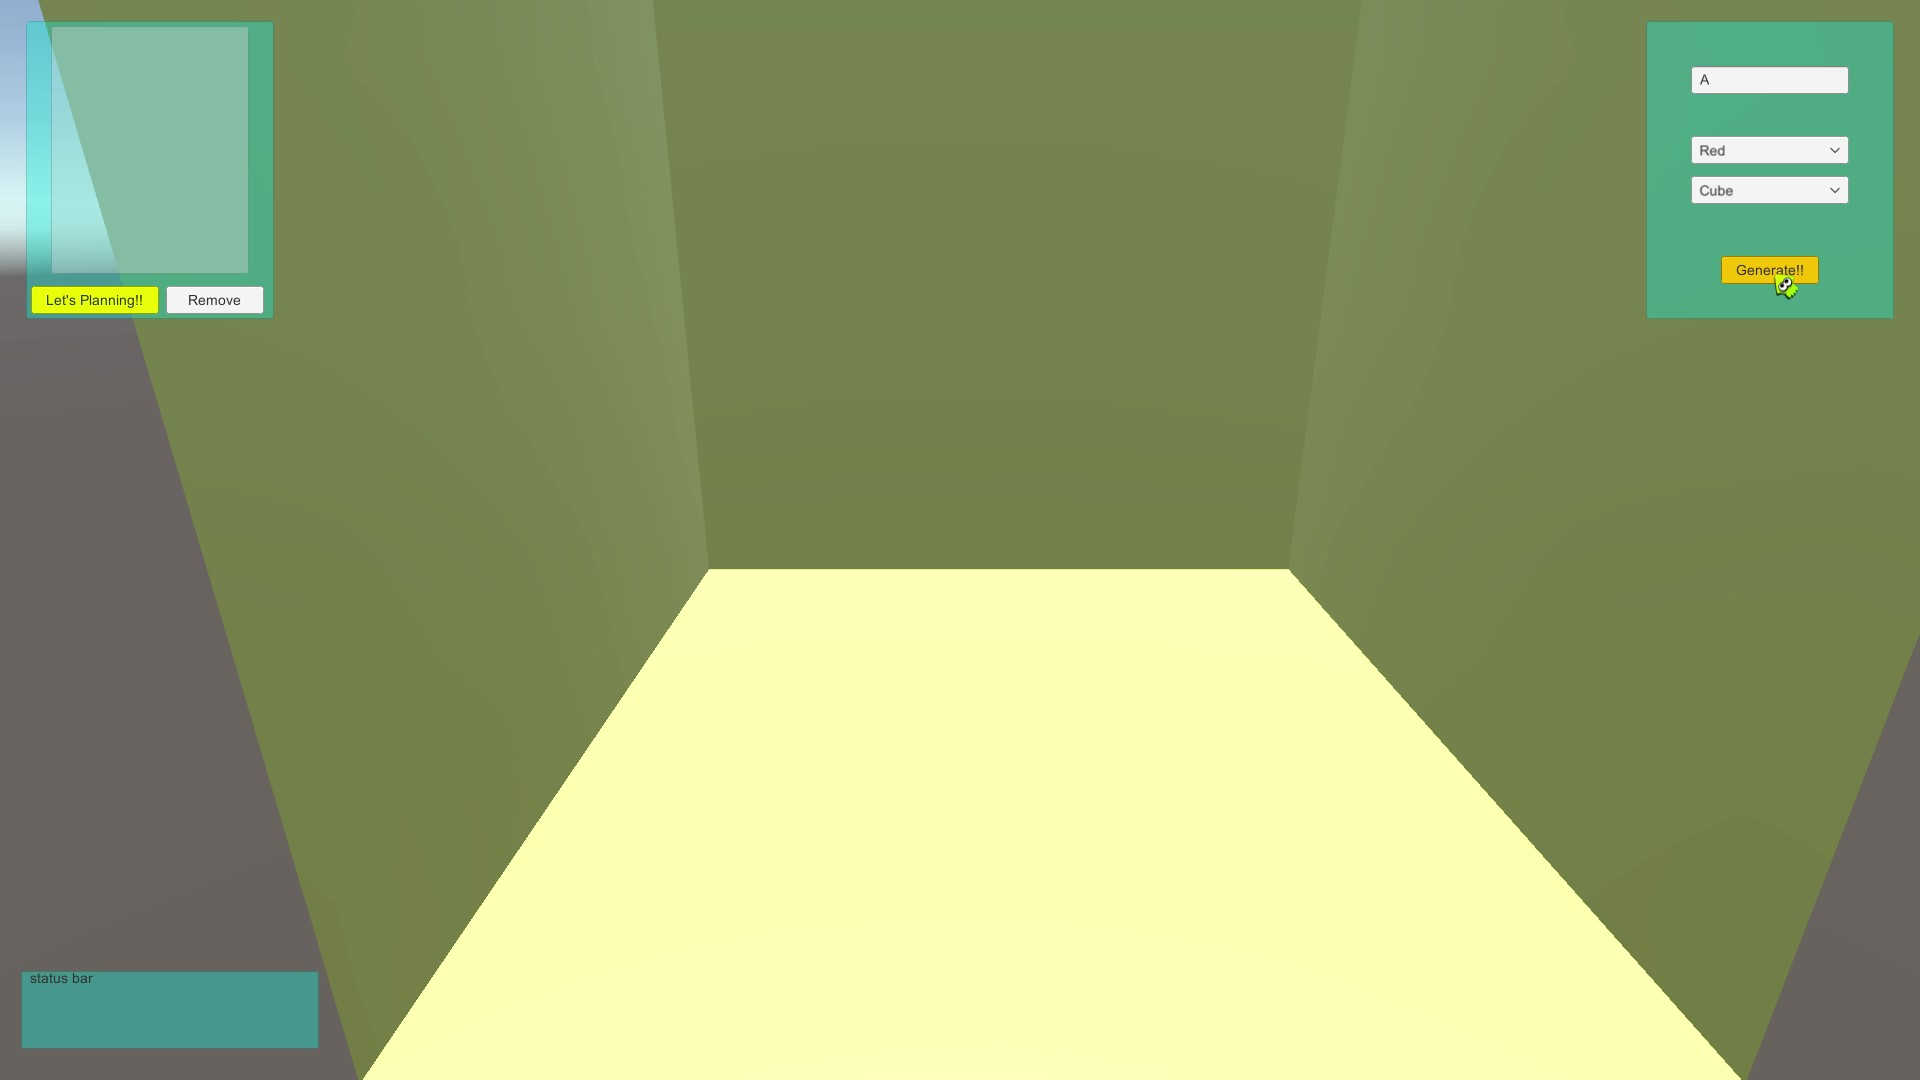
\includegraphics[scale=0.2]{images/BWP_Work6/bwp1.jpg}
  		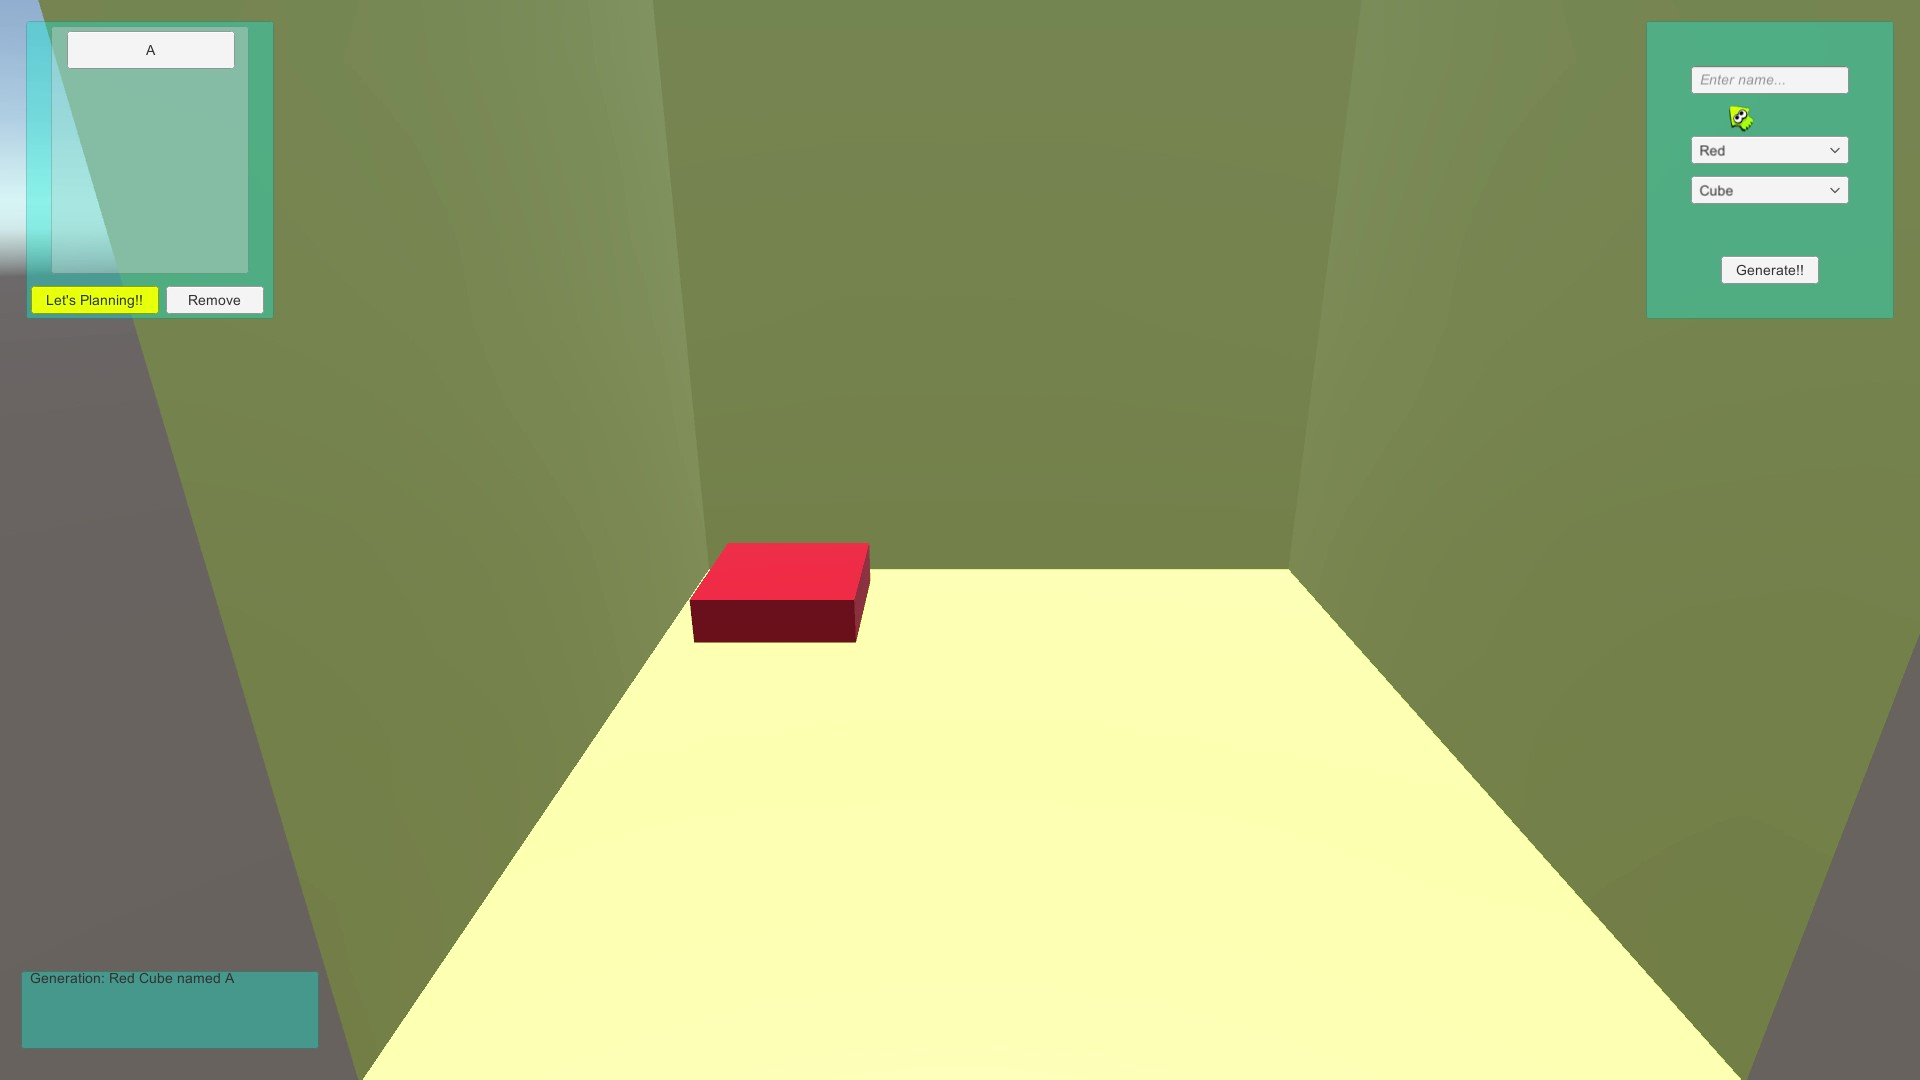
\includegraphics[scale=0.2]{images/BWP_Work6/bwp2.jpg}
	\end{center}
  	\caption{赤い球をAという名前で生成}
  	\label{fig:run1}
\end{figure}

\begin{figure}[!hbt]
  	\begin{center}
  		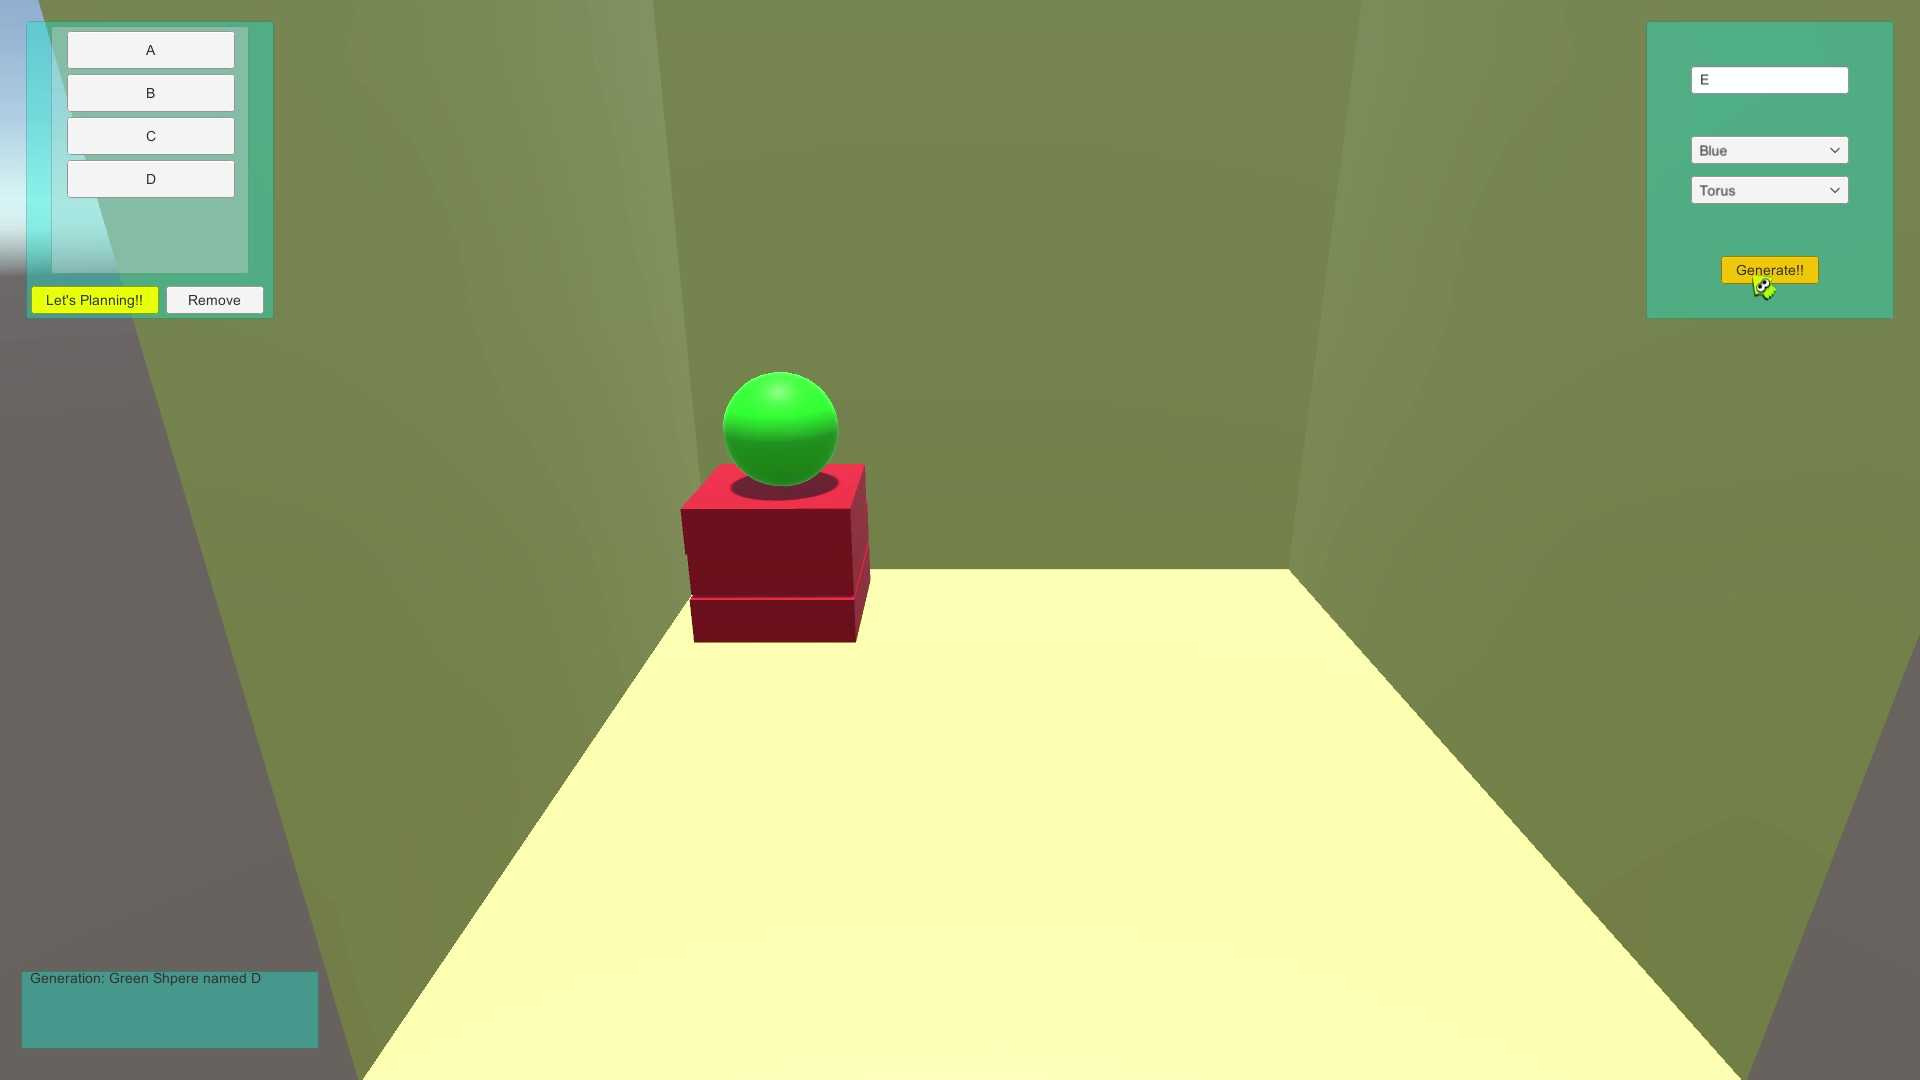
\includegraphics[scale=0.2]{images/BWP_Work6/bwp3.jpg}
  		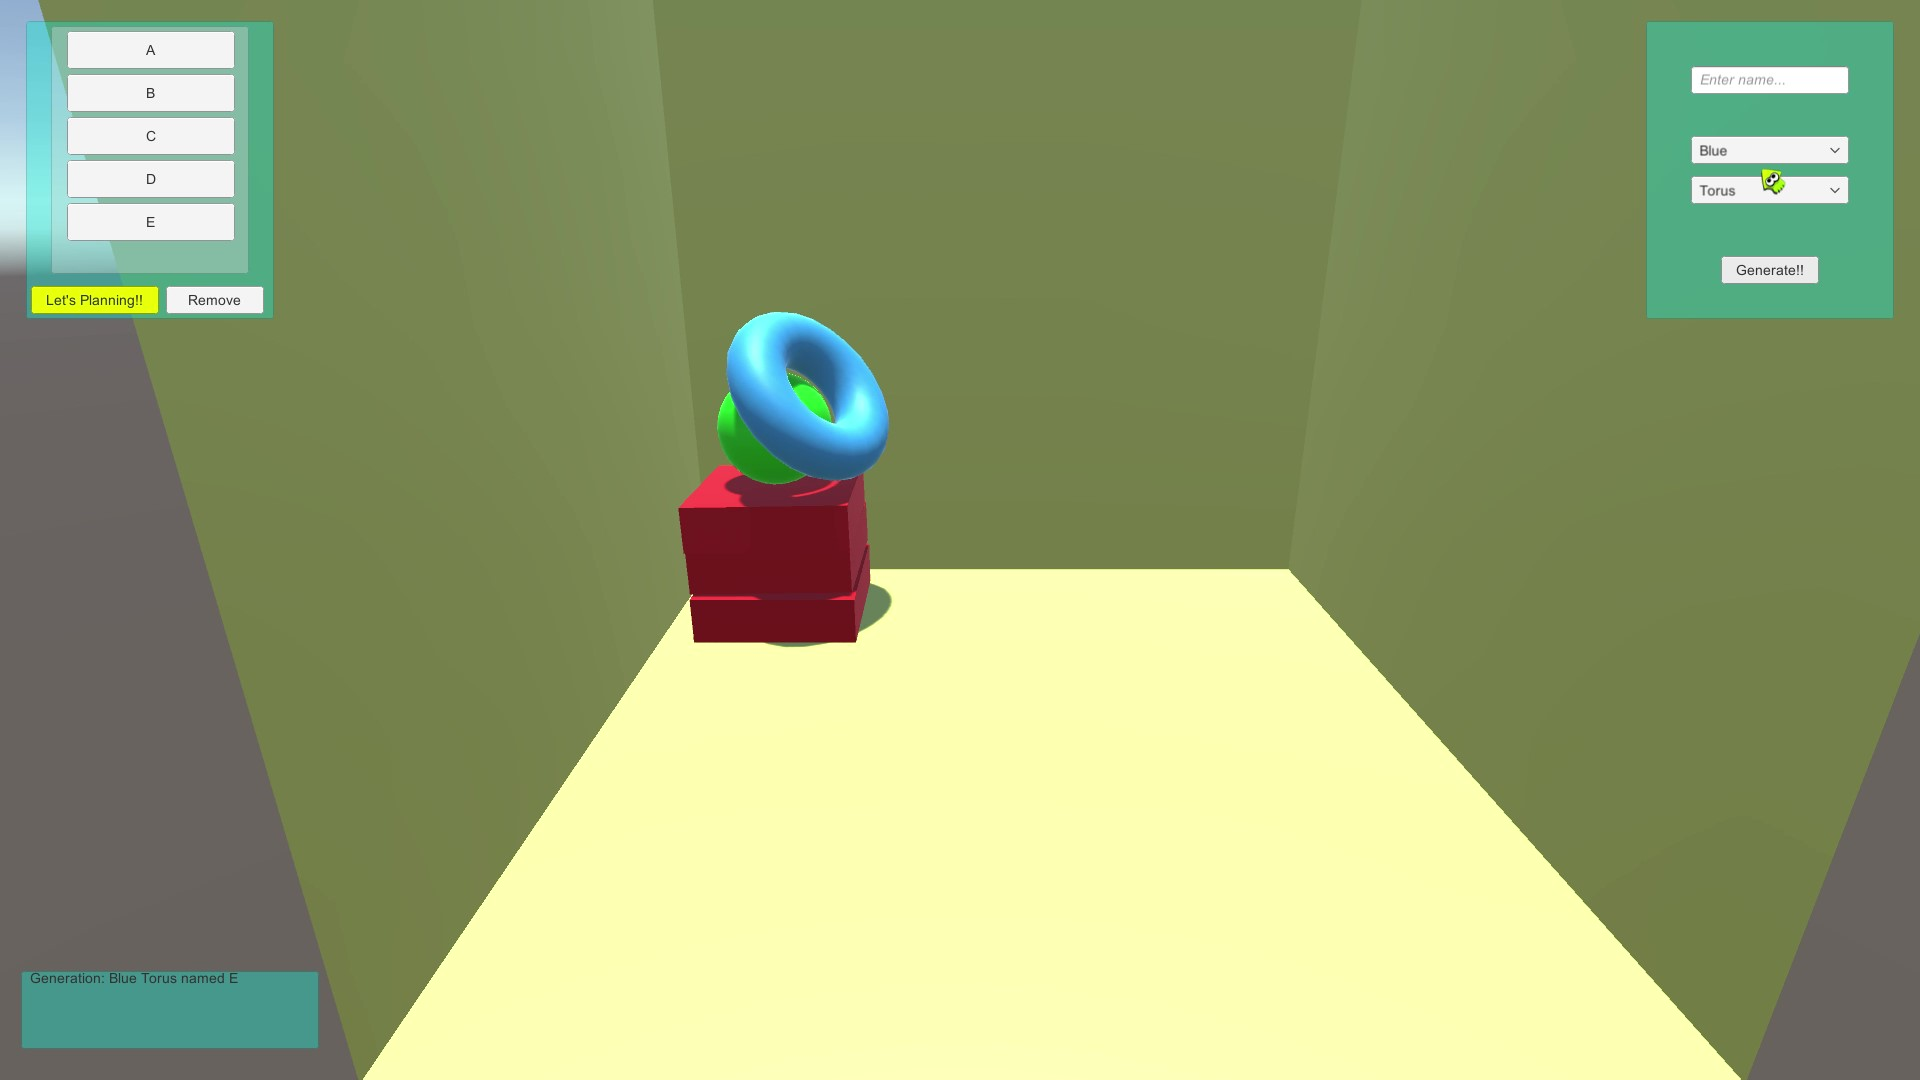
\includegraphics[scale=0.2]{images/BWP_Work6/bwp4.jpg}
	\end{center}
  	\caption{青い円環体をEという名前で生成}
  	\label{fig:run2}
\end{figure}
\clearpage

Preparatorで要素を選択すると,対応するブロックのアウトラインが表示される(図\ref{fig:run3}).

\begin{figure}[!hbt]
  	\begin{center}
  		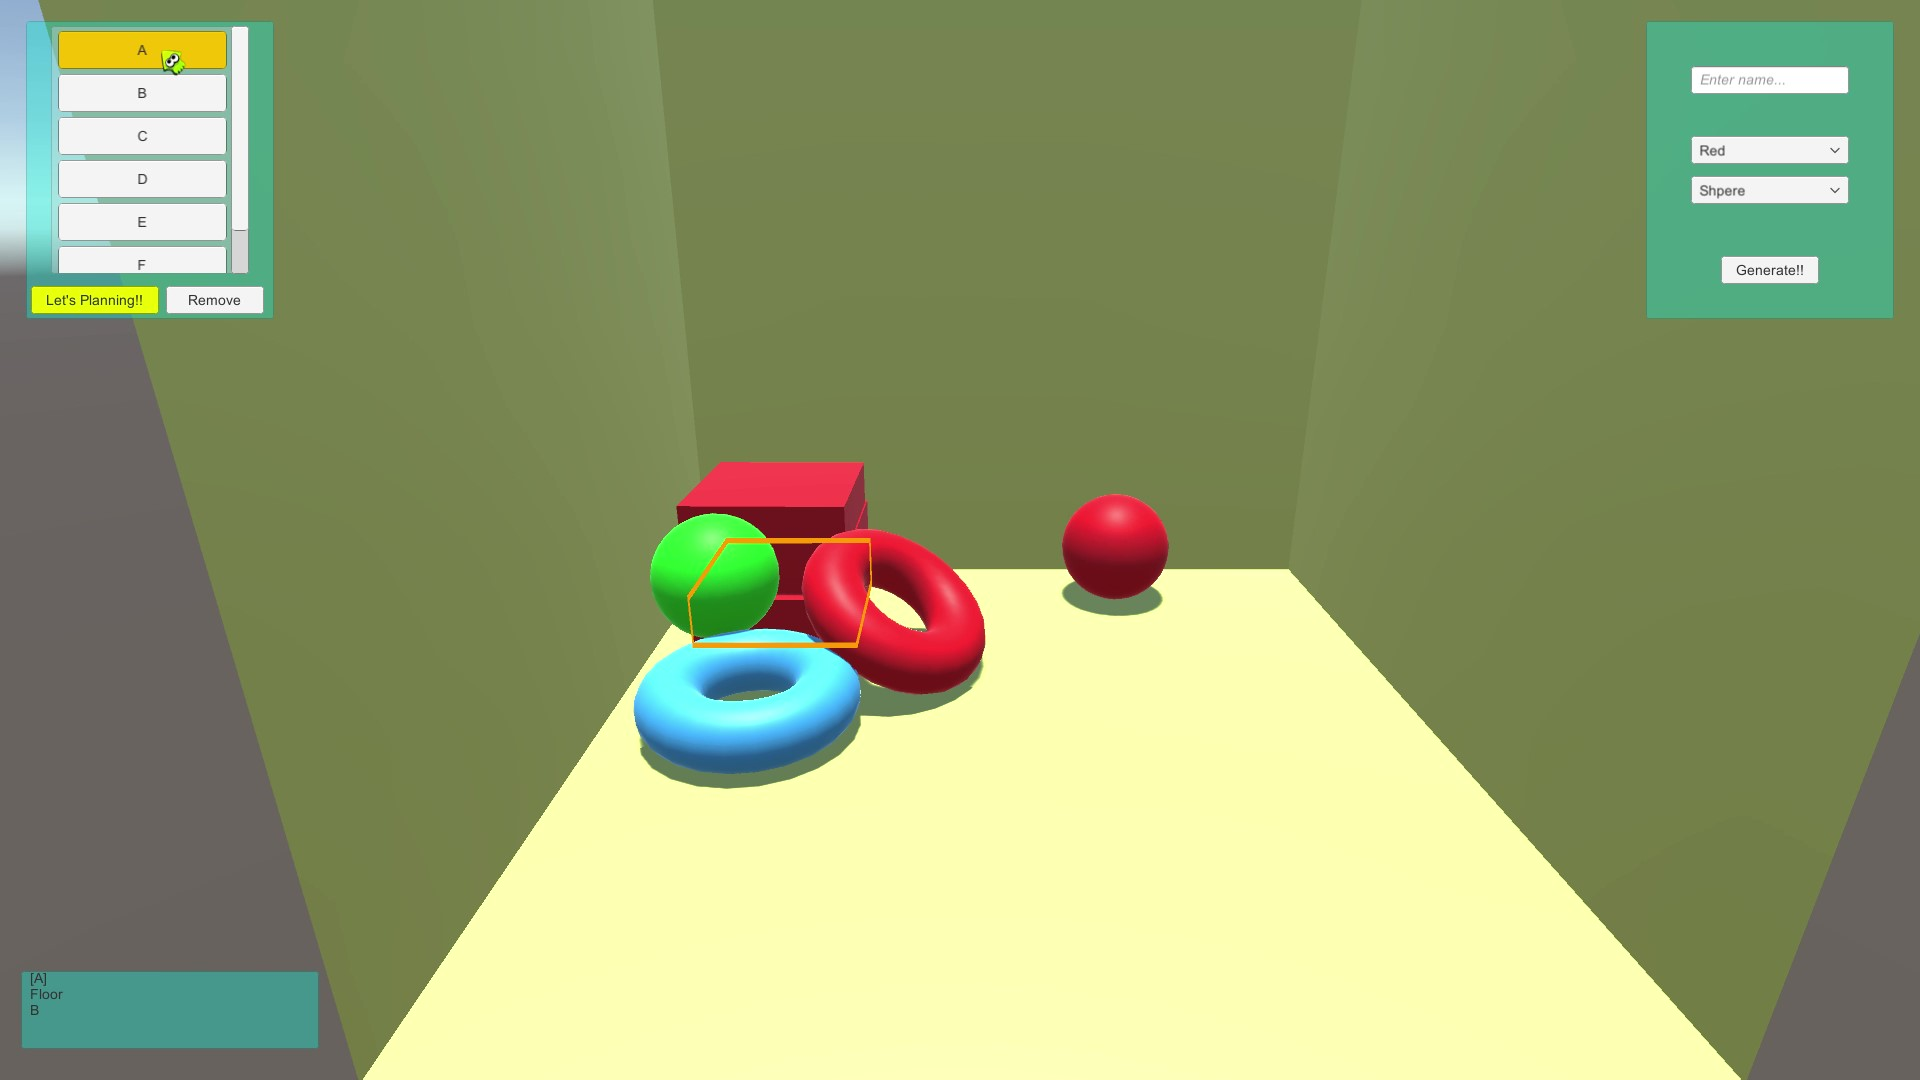
\includegraphics[scale=0.2]{images/BWP_Work6/bwp5.jpg}
	\end{center}
  	\caption{Aにフォーカス}
  	\label{fig:run3}
\end{figure}
\clearpage

フォーカスしたブロックはRemoveボタンで削除できる(図\ref{fig:run4}).

\begin{figure}[!hbt]
  	\begin{center}
  		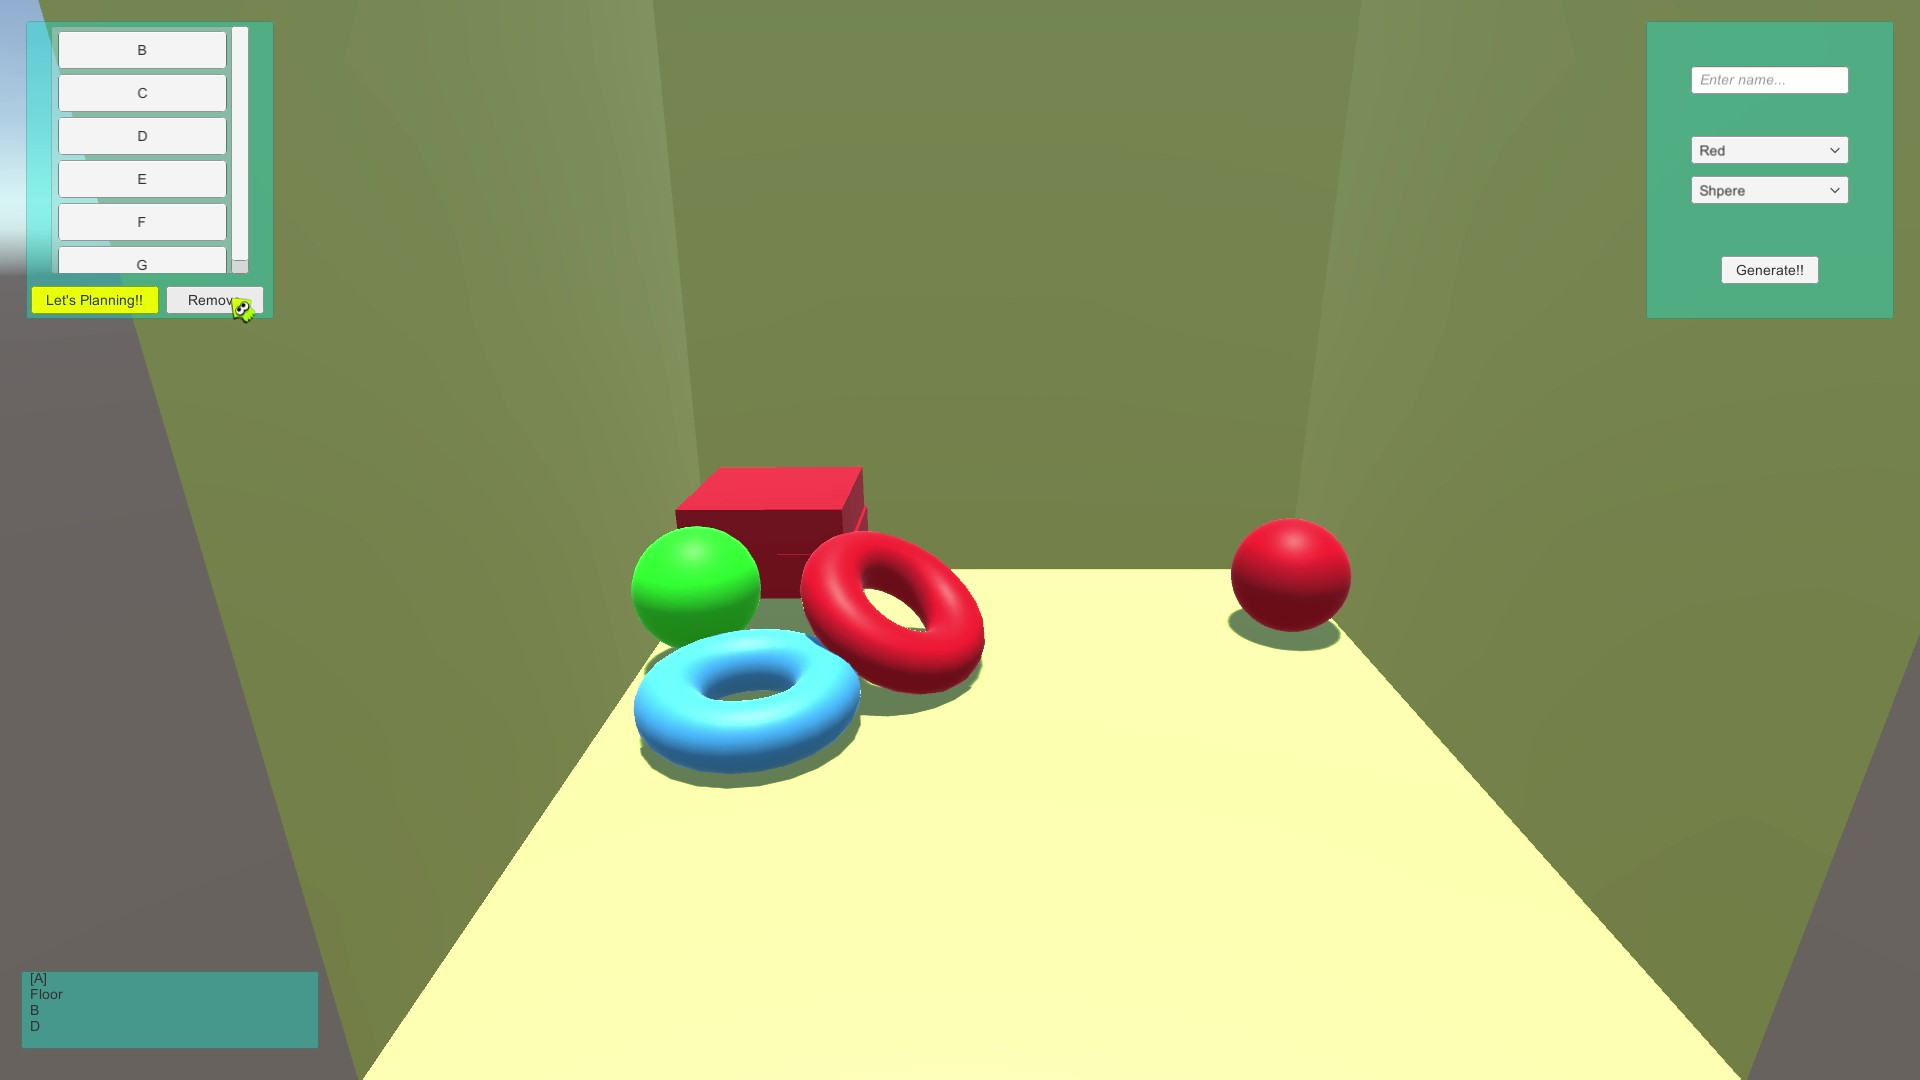
\includegraphics[scale=0.2]{images/BWP_Work6/bwp6.jpg}
	\end{center}
  	\caption{Aを削除}
  	\label{fig:run4}
\end{figure}
\clearpage

ブロックの生成や削除が完了したら,Let's Planningボタンでプランニングを開始する(図\ref{fig:run5}).

\begin{figure}[!hbt]
  	\begin{center}
  		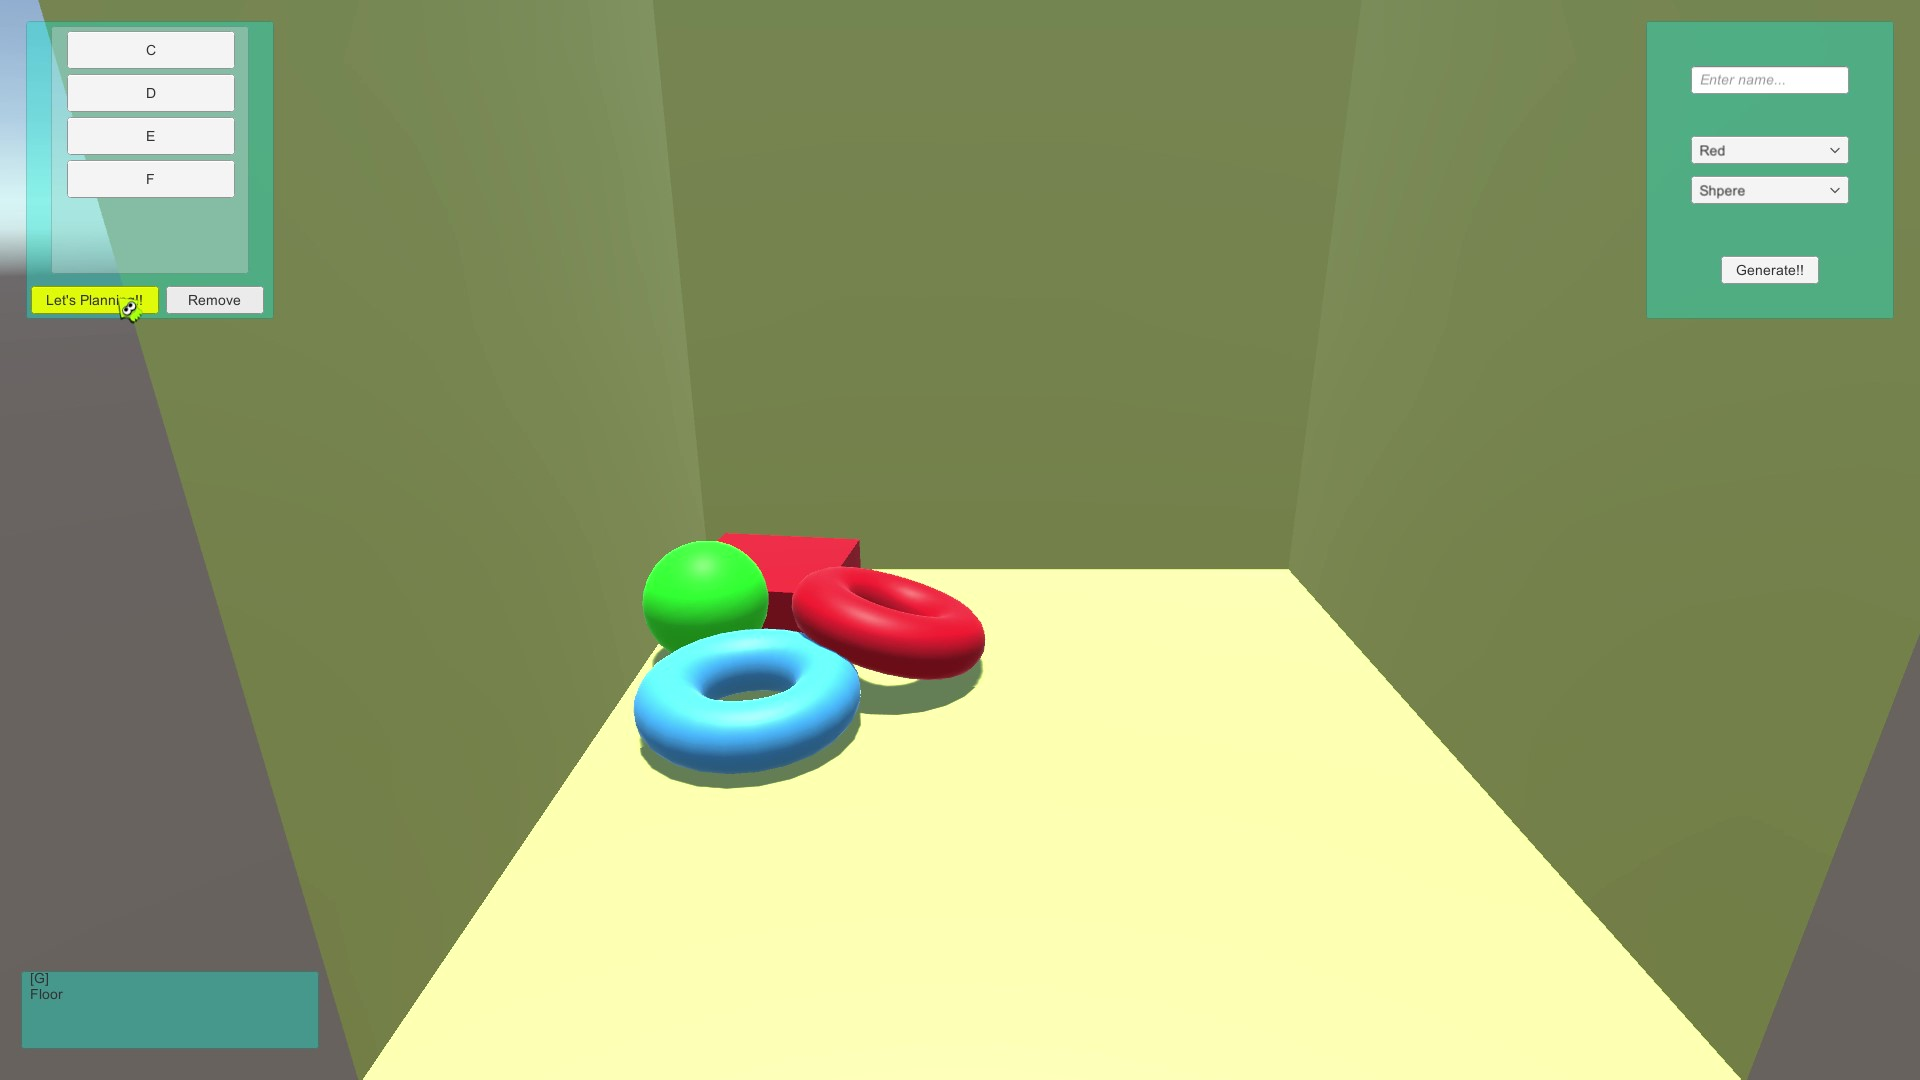
\includegraphics[scale=0.2]{images/BWP_Work6/bwp7.jpg}
	\end{center}
  	\caption{プランニング初期状態}
  	\label{fig:run5}
\end{figure}
\clearpage

フォーカスしたブロックと衝突しているブロックの情報がStaterに表示される(図\ref{fig:run6},\ref{fig:run7}).

\begin{figure}[!hbt]
  	\begin{center}
  		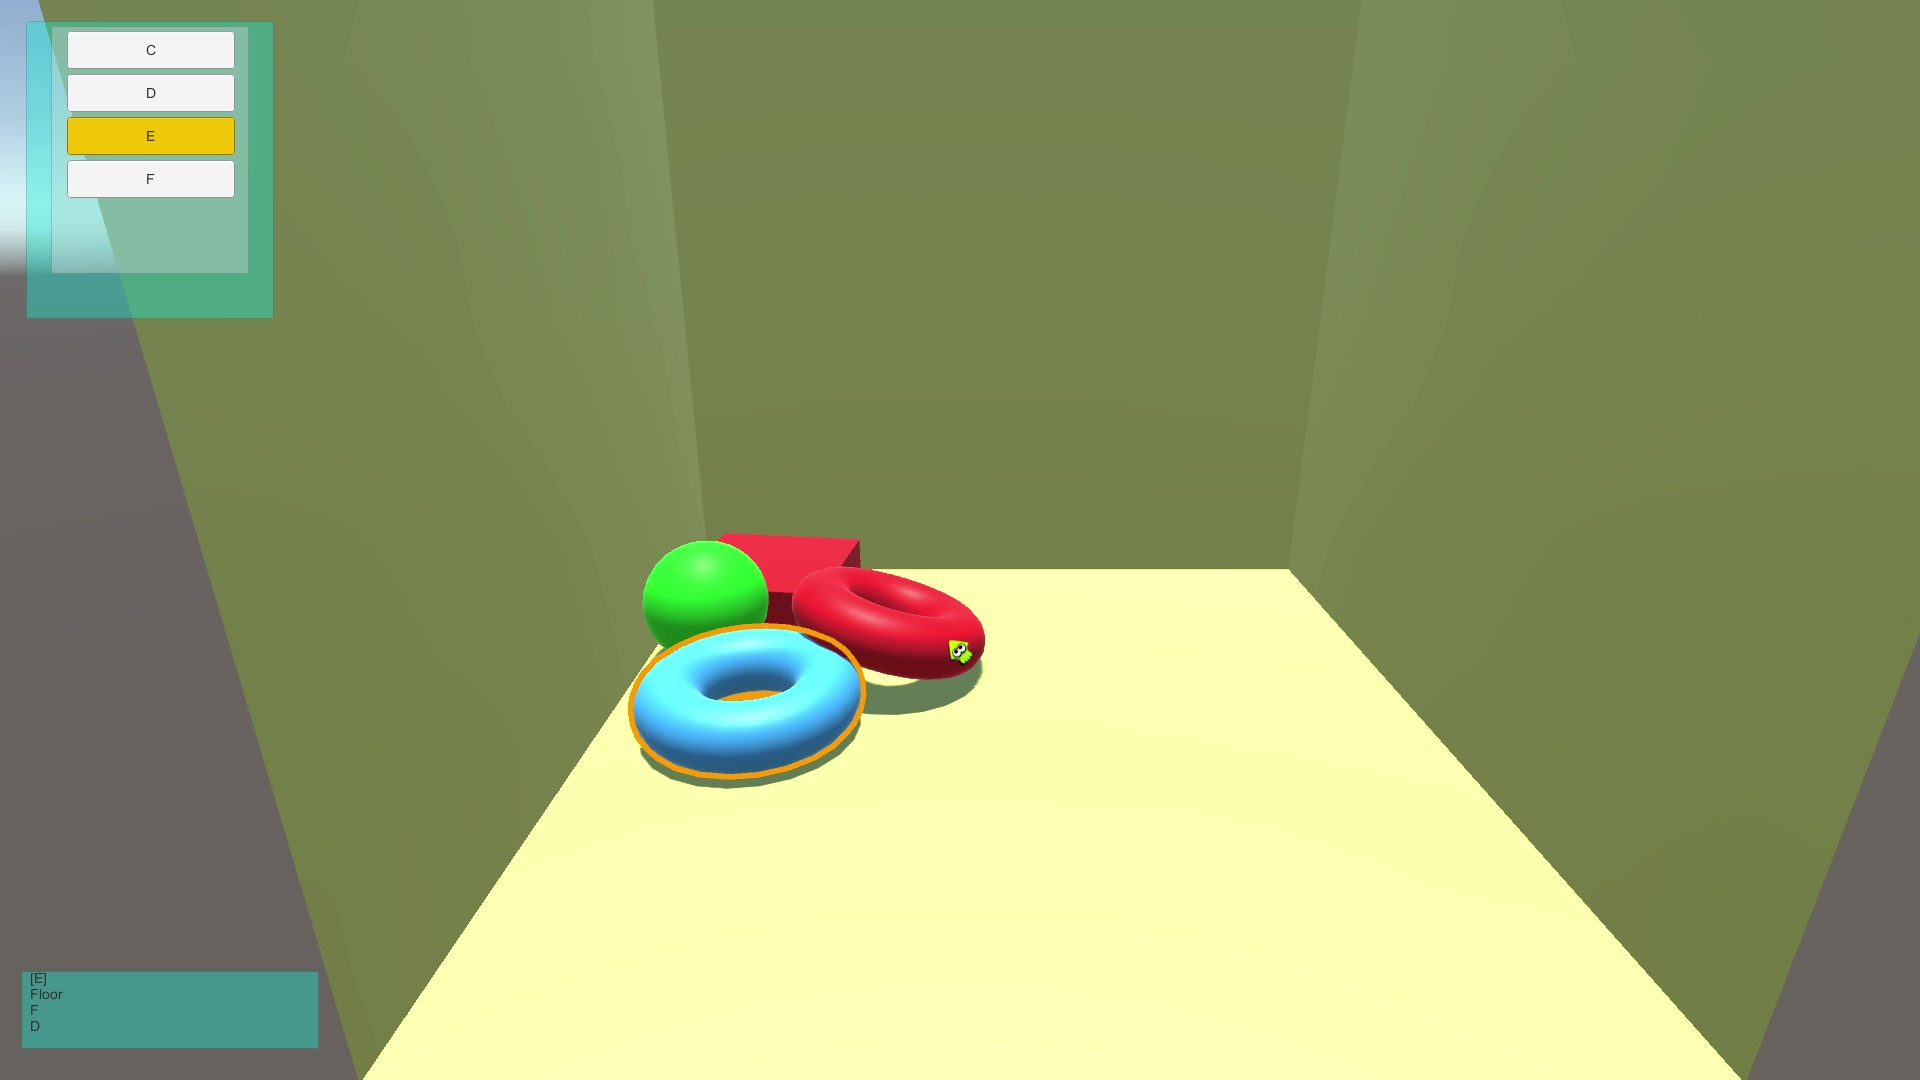
\includegraphics[scale=0.2]{images/BWP_Work6/bwp8.jpg}
  		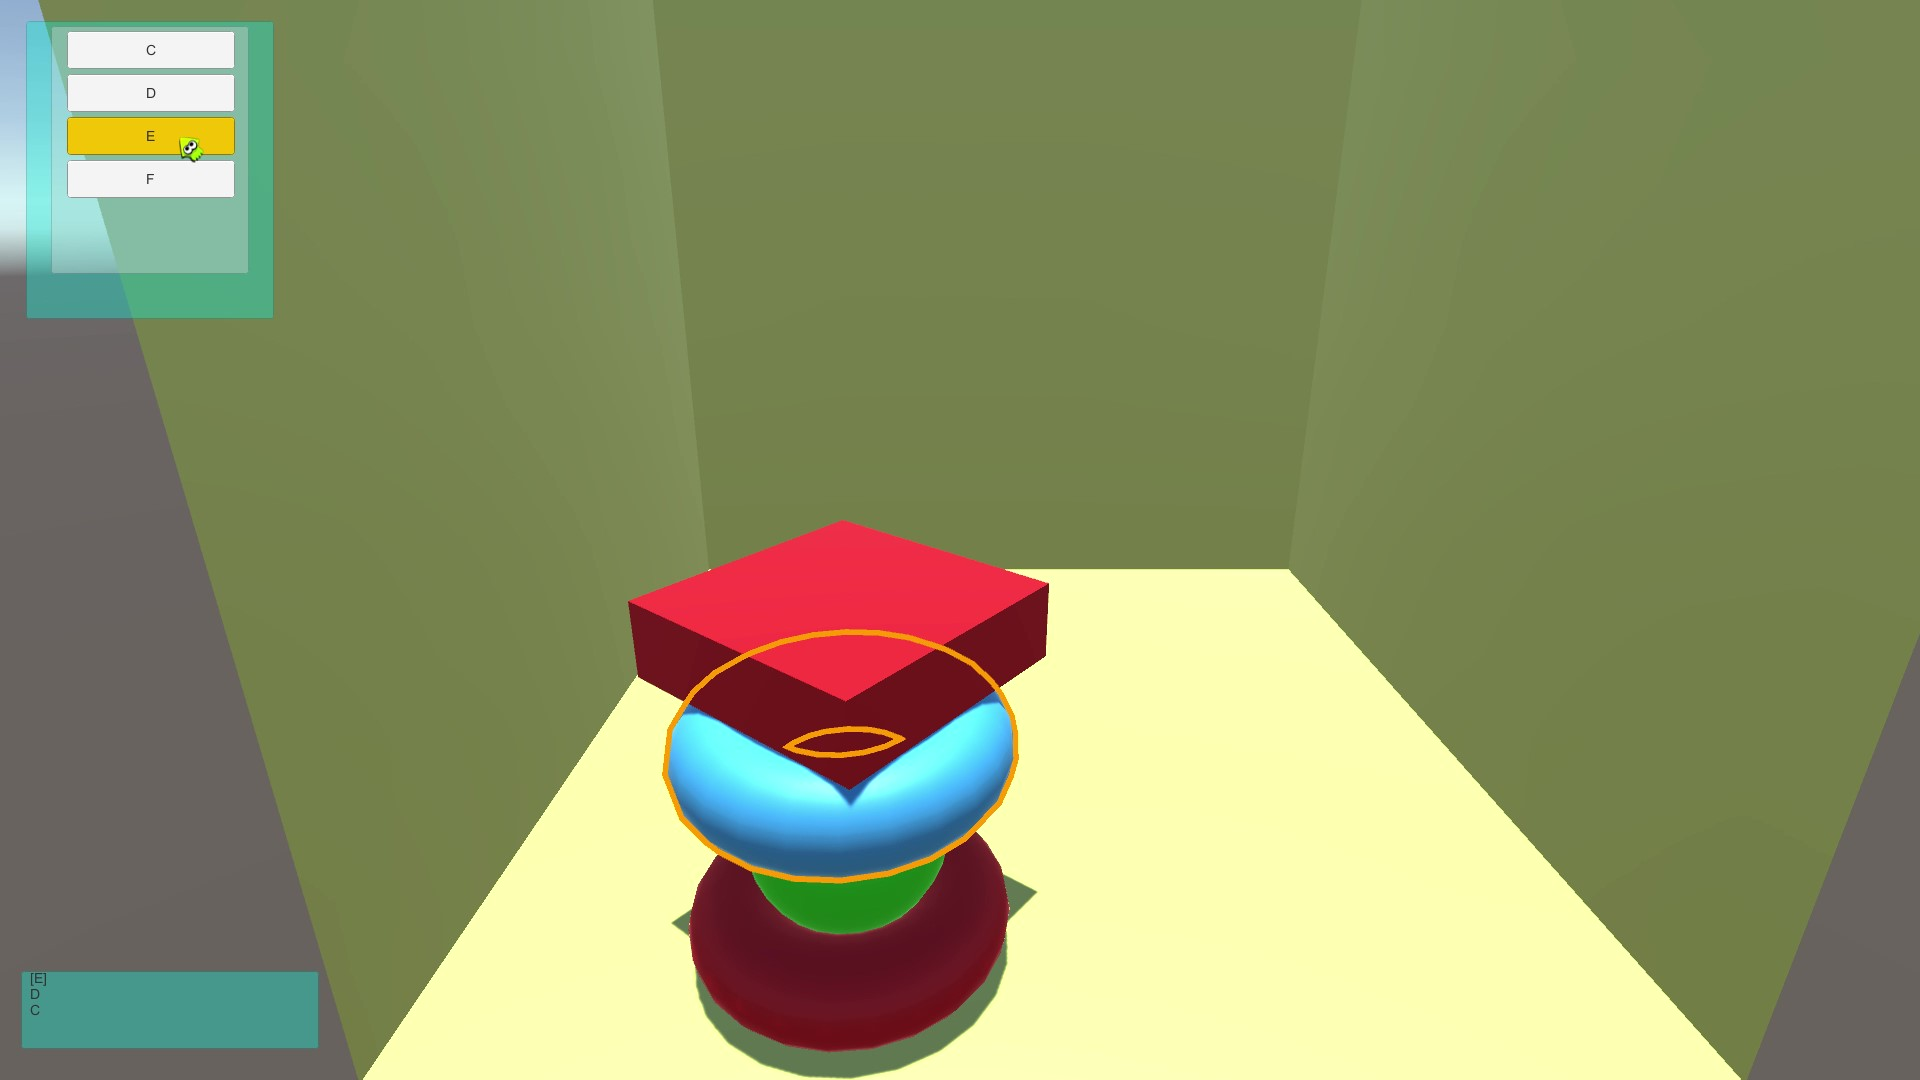
\includegraphics[scale=0.2]{images/BWP_Work6/bwp9.jpg}
	\end{center}
  	\caption{Eにフォーカスを当て,プランニング実行}
  	\label{fig:run6}
\end{figure}

\begin{figure}[!hbt]
  	\begin{center}
  		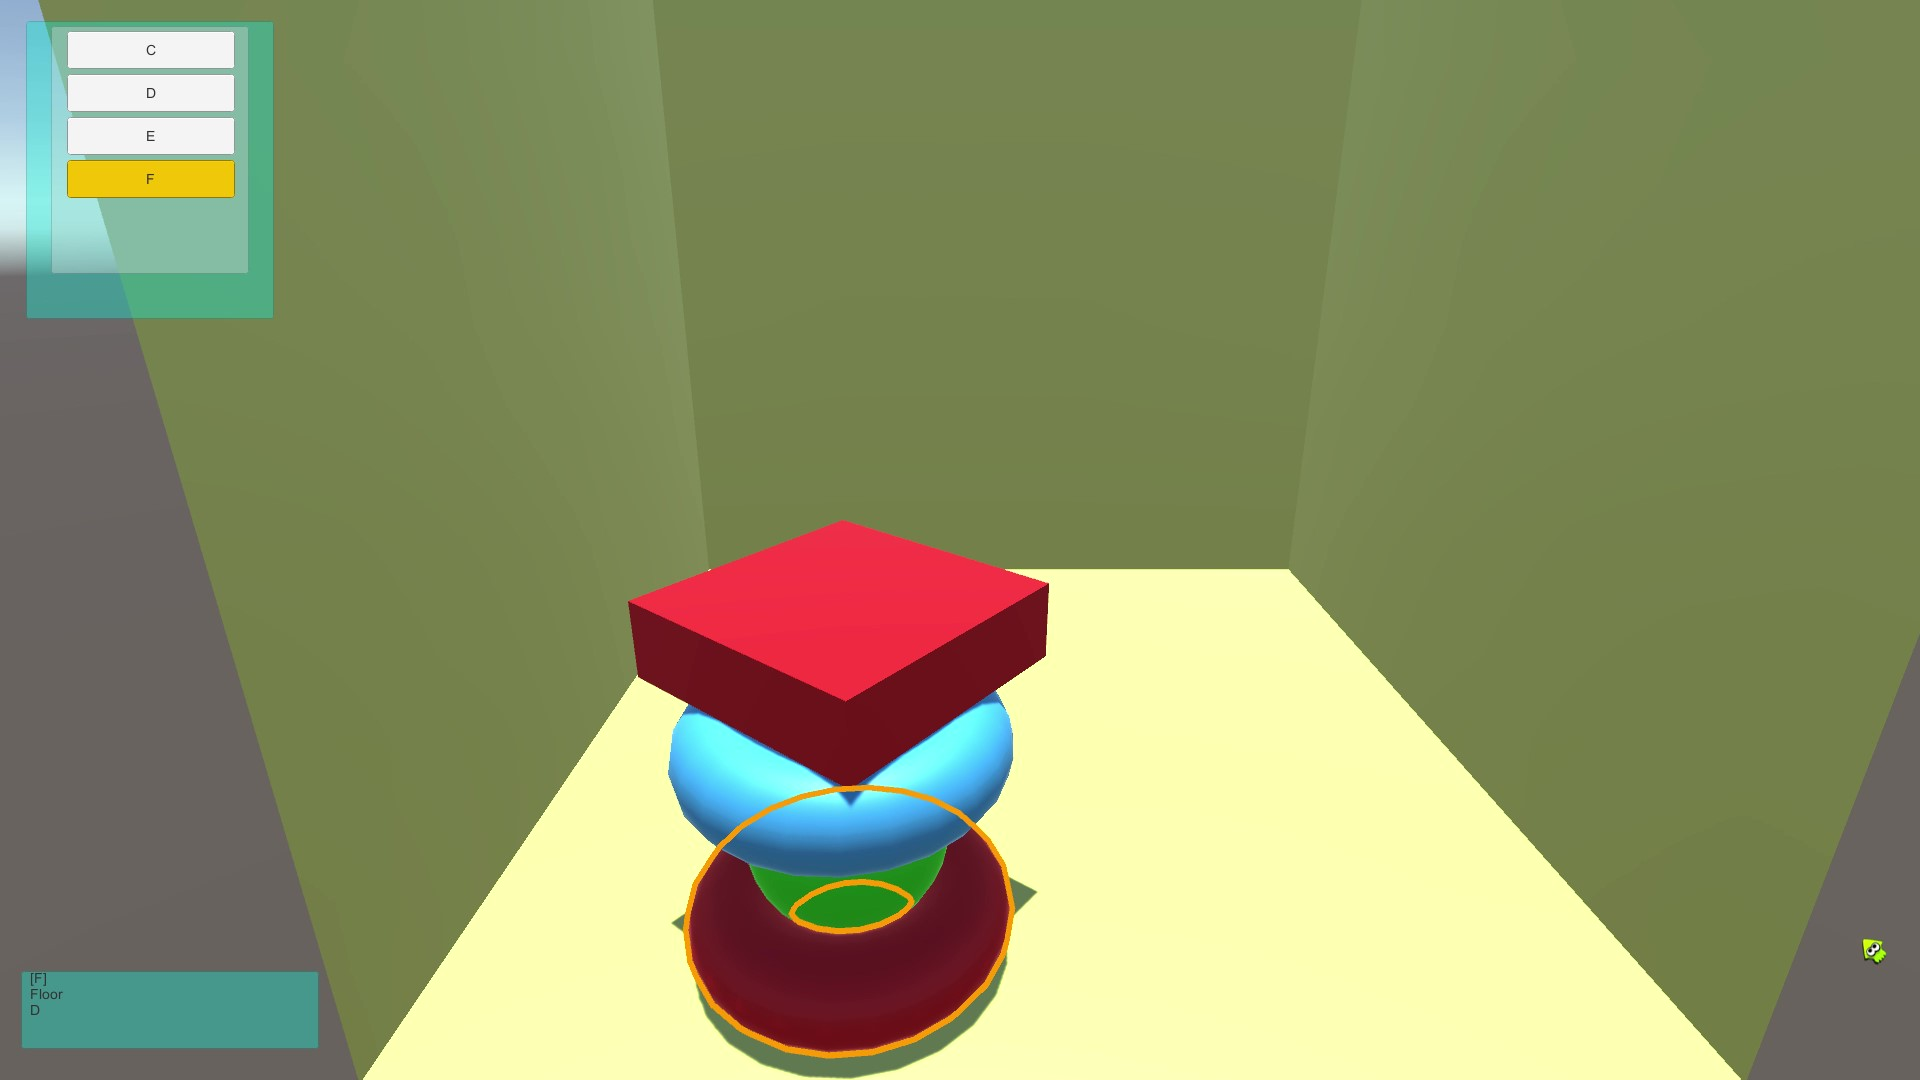
\includegraphics[scale=0.2]{images/BWP_Work6/bwp10.jpg}
  		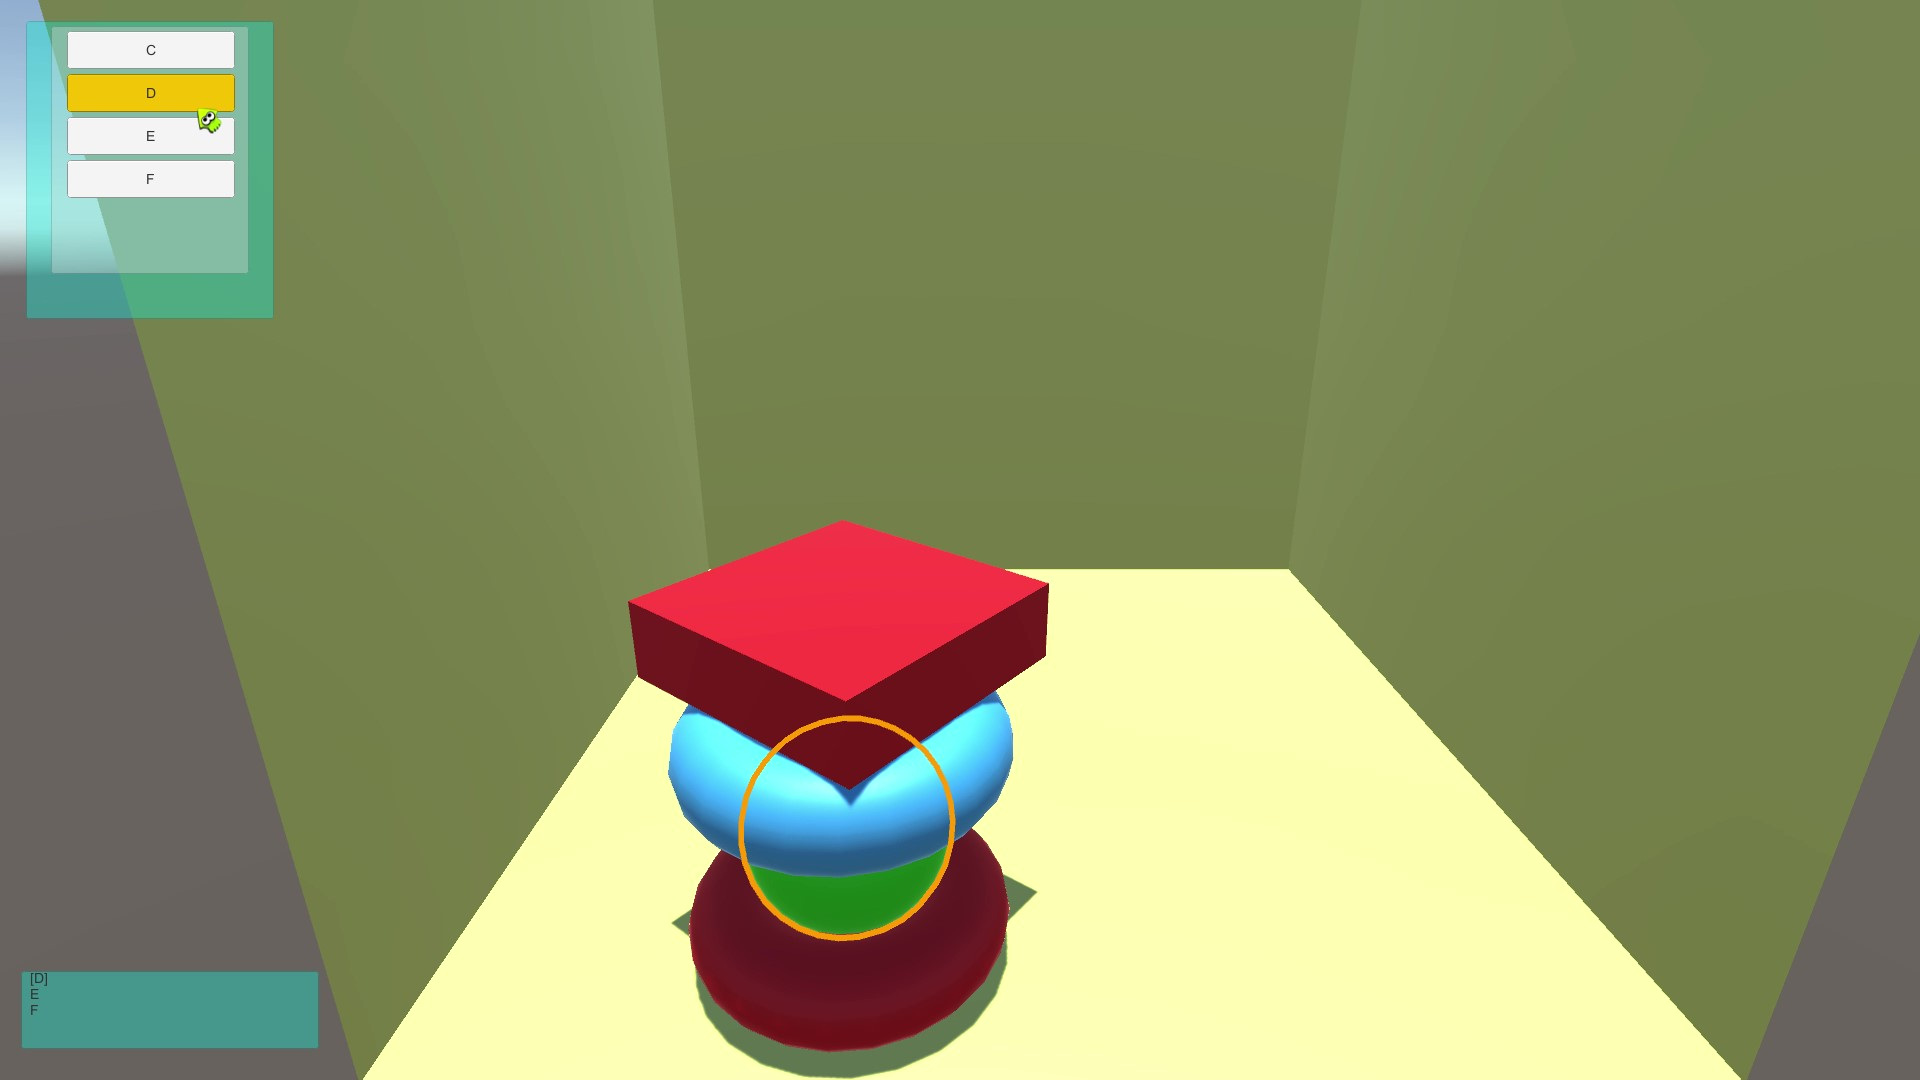
\includegraphics[scale=0.2]{images/BWP_Work6/bwp11.jpg}
	\end{center}
  	\caption{プランニング完了時の各ブロックの衝突情報}
  	\label{fig:run7}
\end{figure}
\clearpage

\subsection{考察}
Generatorスクリプト(ソースコード\ref{src:gen})にて,switchを用いているが,ここで用いる変数objの宣言の際,初期化しないとコンパイルエラーになることはC\#の特徴として挙げられると考えられる.

GUIを実装し始めた際,自動で追加されたEventSystemというオブジェクトを誤って消してしまい,実行してもButtonやInputFieldが全く反応しないという事態に陥った.EventSystemを追加し直すことで修正できたが,このように自動で用意されるものに甘んじて各種機能を使うことは,便利な反面で,何かトラブルが起こったときに簡単には自力で直せないという事態が起こり得ることに繋がるため,自分が利用している機能はどのようなものに基づいてどのように動いているのかを探求することは,今後それを用いてより高度なことをするときのためにも大切なことだと感じた. \\

uGUIでのGUI実装とSwingでのGUIの実装と比較してみると,Swingよりも並列動作は扱いやすく,Swingよりも変数の管理は面倒だと感じた.UnityでのGUIの部品となる各オブジェクトは,常時独立して動き続けているため,並列的な動作を行ったときにどのような挙動をとるかをオブジェクト毎に確認できるため挙動の管理がしやすいのだと考えられる.一方で,各オブジェクトが独立しているということは,オブジェクト間の変数はスクリプトを用意して共有する必要があるということなので,並列動作の分かりやすさと変数の管理の楽さはトレードオフの関係にあることが考えられる.

また,uGUIとSwingのいずれも,フォーカスの操作はとっつき辛いと感じた.しかし,uGUIではGUI全体のフォーカスが1つのEventSystemによって明確に行われているため,その点ではuGUIの方が把握しやすいと感じた.

しかし,GUIの一番の難点は,やはり実行する環境によって表示のされ方が異なってくることだと考えられる.その点では,Swingも標準の機能としてレイアウトが用意されてはいるが,uGUIでのアンカーを用いた配置の方が,断然とっつきやすく,調整もしやすいと感じた.

以上のことから,今後GUIを作る際は,基本的にSwingよりもuGUIで良いと考えられる.しかし,軽量化という点においてuGUIはSwingに優ることができるか,または優る必要があるかということは今後の課題である. \\

Unityを使って一番悩まされたことが,プレハブにアタッチしたコンポーネントの変数がpublicでも,その変数に他のオブジェクトを直接アタッチして参照させることができなかったことである.そのため,GameObject.Findメソッドで毎度目的のオブジェクトを探して参照を作っているが,直接アタッチできる方が効率的だと考えられる.前回も,通常のオブジェクトだと上手くいくのにプレハブだとうまくいかないようなこと(Torusの衝突判定)があったように,ブレハブの特性や注意点で理解できていないことがまだ多々あることが考えられる.Unityを使っていく上でプレハブは欠かせない機能なので,今後も積極的に使って学んでゆきたい.

また,Unityではオブジェクトを消去するという機能があるため,この点も注意して使っていかなければいけないと考えられる.Unityに限らず並列処理を行うようなプログラムでは,先程まで参照していたものが突然なくなるということが往々にして起こり得るため,その点も留意した上でのプログラム実装を行ってゆく必要があると考えられる.

また,Unityにおいて,変数をオブジェクト間で共有するために,いちいちスクリプトを作成する必要があると述べたが,共有する変数ごとにスクリプトを作成するのではなく,共有すべき変数をまとめて管理するようなスクリプトと,そのためのオブジェクトを作成して,そこを共有変数の仲介場所とすると改善できることが考えられる.例えば,今回のプログラムではStaterがその仲介場所として適していたと考えられる.更に,Staterを仲介場所にすればステータスの表示もより自在に行えるようになることが考えられ,一石二鳥である.また,このような方法で共有する変数を管理したほうが,プログラムの保守性的にも良いということが考えられる. \\

今回の実装について,開始時点を決めれるようにしたことで,初期状態の明確化ができるようになった.

最終的に自動でのプランニングを実装するには,その前段階として実装する必要のあるものが多くあったため,その過程の一部を実装しようと思い今回作ったような実装となった.
ブロックの属性付与や生成したブロックの管理,衝突情報の管理が行えるようにしたことで,プランニング実装に向けて次に必要なのは,衝突情報を突き詰め,どちらのブロックが上に乗っているかといった相対的な位置関係の取得・管理をすることと,それに基づきどの物体を目標状態に向けてどう動かすかを選択することの実装だと考えられる.
しかし,3次元空間における物体間の衝突の仕方は多様であり,どちらのブロックが上に乗っているかを厳密に判別することは困難な場合が多く存在することが考えられる.また,それを解決したところで,物体を動かすことによる状態変化も不定であり,目標状態に向けた行動の選択を一意的に決めることは難しいと考えられる.このように,実装上の難しさだけでなく,そもそも3次元空間上においてどのようにプランニングを定義するかという実世界的な難しさが数多くあることを改めて痛感した.


\section{感想}
グループみんなで協力して,最後までやりきれて良かった.

8班サイコー!!

\begin{thebibliography}{99}
\bibitem{notty} Javaによる知能プログラミング入門 --著:新谷 虎松
\bibitem{notty} 知識システムの実装基礎 --著:新谷 虎松
\bibitem{notty} 人工知能の基礎知識 --著:太原 育夫
\bibitem{notty} LATEX2ε 美文書作成入門 --著:奥村 晴彦

\bibitem{Java新} 新谷虎松『Javaによる知能プログラミング入門』コロナ社,2002年.
\bibitem{Swing} Let'sプログラミング Swingを使ってみよう, \url{https://www.javadrive.jp/tutorial/} (2019年1月3日アクセス).

\bibitem{notty} Javaによる知能プログラミング入門 --著:新谷 虎松

\bibitem{unity} Unity Technologies.: 『Unity - Manual: Unity User Manual (2019.2)』 https://docs.unity3d.com/Manual/index.html (2020/01/06アクセス)
\bibitem{ugui} 竹内 大五郎: 『uGUIチュートリアル - Metal Brage』 http://www.metalbrage.com/UnityTutorials/uGUI/index.html (2020/01/06アクセス)
\bibitem{sv} shimoaraiso: 『UnityのScrollViewで一覧表示を作成する』 https://tech.pjin.jp/blog/2016/08/30/unity\_skill\_3/ (2020/01/06アクセス)
\bibitem{outline} chrisnolet: 『chrisnolet/QuickOutline: Unity asset for adding outlines to game objects』 https://github.com/chrisnolet/QuickOutline (2020/01/06アクセス)
\bibitem{sb} hiyotama: 『【Unity開発】uGUIのScrollbarの使い方【ひよこエッセンス】 - Unity(C\#)初心者・入門者向けチュートリアル ひよこのたまご』 https://hiyotama.hatenablog.com/entry/2015/07/04/090000 (2020/01/06アクセス)
\bibitem{latex} PukiWiki Developers Team.: 『【LaTeX入門/相互参照とリンク - TeX Wiki』 https://texwiki.texjp.org/?LaTeX?LaTeX入門\%2F相互参照とリンク\#h84e81eb (2020/01/06アクセス)
\end{thebibliography}

\end{document}
